%%
%% 研究報告用スイッチ
%% [techrep]
%%
%% 欧文表記無しのスイッチ(etitle,eabstractは任意)
%% [noauthor]
%%

%\documentclass[submit,techrep]{ipsj}
\documentclass[submit,techrep,noauthor]{ipsj}


% \usepackage[dvips]{graphicx}
\usepackage[dvipdfmx, hiresbb]{graphicx}
\usepackage{latexsym}
\usepackage{amsmath}
\usepackage{enumitem}
\usepackage{amssymb} 
\usepackage{url}
\usepackage{xcolor}

\newcommand{\todo}[1]{\colorbox{yellow}{{\bf TODO}:}{\color{red} {\textbf{[#1]}}}}
\newcommand{\ihara}[1]{\colorbox{green}{{\bf IHARA}:}{\color{blue} {\textbf{[#1]}}}}
\newcommand{\memo}[1]{\colorbox{magenta!30}{\textbf{MEMO}}{\color{red!50}\textbf{[#1]}}}

\def\Underline{\setbox0\hbox\bgroup\let\\\endUnderline}
\def\endUnderline{\vphantom{y}\egroup\smash{\underline{\box0}}\\}
\def\|{\verb|}
%

%\setcounter{巻数}{59}%vol59=2018
%\setcounter{号数}{10}
%\setcounter{page}{1}


\begin{document}


\title{強化学習を用いたScratchにおける\\
リミックス元作品のCTスコア予測}

% \etitle{How to Prepare Your Paper for IPSJ SIG Technical Report \\ (version 2018/10/29)}

\affiliate{WU}{和歌山大学\\
Wakayama University, 930 Sakaedani, Wakayama 640--8510, Japan}



\author{堀尾 桃夏}{Horio Momoka}{WU}[momo5588.school@gmail.com]
\author{伊原 彰紀}{Ihara Akinori}{WU}[ihara@wakayama-u.ac.jp]

\begin{abstract}
本研究は,ビジュアルプログラミング言語Scratchにおいて,リミックス元作品のコンピュテーショナル・シンキング(CT)スコアを予測する手法を提案する.
Scratchが有する他者の作品を複製・編集するリミックス機能が,学習者のCTスコア向上に有効であることが知られるが,その効果はユーザの学習経験によって異なることが従来研究で示されている.
本研究では,Scratchユーザがこれから制作する作品が,過去に制作した作品のCTスコアを上回ることに寄与する,リミックス対象作品のCTスコアを予測するモデルを構築する.
具体的には,作品の制作過程をマルコフ決定過程として捉え,強化学習を用いてユーザの学習経験に応じてリミックスした元の作品のCTスコアを予測するモデルを構築する.評価実験の結果,提案モデルは,CTスコアが低い初級者において,CTスコア向上に有効であることを確認した.
\end{abstract}


%
\begin{jkeyword}
    {Scratch,ビジュアルプログラミング,強化学習}
\end{jkeyword}
%

%\begin{eabstract}
%This document is a guide to prepare a draft for submitting to IPSJ
%Journal, and the final camera-ready manuscript of a paper to appear in
%IPSJ Journal, using {\LaTeX} and special style files.  Since this
%document itself is produced with the style files, it will help you to
%refer its source file which is distributed with the style files.
%\end{eabstract}
%
%\begin{ekeyword}
%IPSJ Journal, \LaTeX, style files, ``Dos and Dont's'' list
%\end{ekeyword}

\maketitle

%%%%%%%%%%%%%%%%%%%%%%%%%%%
\section{はじめに}
%%%%%%%%%%%%%%%%%%%%%%%%%%%

日本では2020年度から小学校のプログラミング教育の必修化,2021年度から中学校のプログラミングに関する内容の充実,2022年度から高等学校において共通必履修科目「情報1」が新設されている\cite{monkashou}.しかし,指導者の情報不足や人材不足,予算不足などの指導者に対する問題が複数挙げられている\cite{monkashou2}.日本よりも早い時期からプログラミング教育を開始しているアメリカでは,プログラミング初学者向けのビジュアルプログラミングScratch\footnote{Scratch:\url{https://scratch.mit.edu/}}\cite{resnick2009scratch}を用いてプログラミング教育を行っている.Scratchは「繰り返す」などの命令処理をもつブロックを,ジグソーパズルのように組み合せることで作品を完成させる.さらに,完成した作品はオンライン上に公開することができ,公開されている他ユーザの作品は,見る,使うだけでなく,リミックスと呼ばれる機能として,作品を複製し,編集することが可能である.

プログラミング初学者が取り組みやすいScratchは,コンピュテーショナル・シンキング (CT) \cite{wing2006computational}スキルの向上を目的とし,多くの実験で有用性が確認されている\cite{10.1145/2724660.2724674}\cite{hashitani2022scratch}\cite{10.1145/2818048.2819984}.ビジュアルプログラミングは学習や操作のハードルが低いため,プログラミングの入門学習として有効である\cite{1050845762811356288}.また,バグの混入が少なく,直観的な操作のみでプログラミングをすることができるため,ユーザが短期間で作品を完成させやすく,達成感を得やすいという特徴をもつ.
% 近年では,情報化社会の進展に伴い,プログラマー不足が深刻な問題となっている.ビジュアルプログラミング言語の活用はその課題解決の第一歩になると考えられる.
しかし,Scratchをはじめとするビジュアルプログラミングは,ユーザが自由に作品制作するため,明確なカリキュラムは存在せず,プログラミングを通して身につけたCTを自己評価することは困難である.Morenoらは作品に使用されているブロックに基づき,CTスコアを計測するDr.Scratchを開発している\cite{moreno2015dr}.Dr.Scratchは,論理,制御フロー,同期,抽象化,データ表現,ユーザ対話性,並列処理の7つの概念に基づいて作品を評価する.また,各概念を0点から3点の合計21点とし,CTスコアとして評価する.表\ref{CTscoreTable}に各概念の評価方法を示す.CTスコアを3つの区分に分類し,0点から7点をBasic,8点から14点をDeveloping,15点から21点をMasterとして評価する.
% 本論文ではDr.Scratchを用いて,CTスキルを定量的に評価する.

%--------------------------
\begin{table*}[t]
    \centering
    \caption{CT概念とその評価方法\cite{hashitani2022scratch}}
    \label{CTscoreTable}
    \scalebox{0.8}{
    \begin{tabular}{c|c|c|c|c}
    \hline
    CTスキルの概念 & 0点 & 1点 & 2点 & 3点
    \\ \hline
    抽象化 & - &
    \begin{tabular}{c}
    2つ以上の\\スクリプトを使用
    \end{tabular}
    & 定義ブロックを使用 & クローンブロックを使用
    \\ \hline
    並列処理 & - & 
    \begin{tabular}{c}
    緑の旗ブロックを\\2個以上使用 
    \end{tabular}
    & 
    \begin{tabular}{c}
    オブジェクトへのクリックにより\\2つ以上のスクリプトを\\同時に実行する機能を実装
    \end{tabular}
    & 
    \begin{tabular}{c}
    イベント動作により\\2つ以上のスクリプトを\\同時に実行する機能を実装
    \end{tabular}
    \\ \hline
    論理 & - & Ifブロックを使用 & If elseブロックを使用 & 論理演算ブロックを使用
    \\ \hline
    同期 & - & 待機ブロックを使用 &
    \begin{tabular}{c}
    メッセージ受信により\\プログラムを停止する機能を実装
    \end{tabular}
    &
    \begin{tabular}{c}
    指定条件を満たすまで\\プログラムを停止する処理を実装
    \end{tabular}
    \\ \hline
    フロー制御 & - &
    \begin{tabular}{c}
    2個以上の処理ブロックを\\連結して使用
    \end{tabular}
    &
    \begin{tabular}{c}
    指定回数/回数無制限の\\繰り返しブロックを使用
    \end{tabular}
    &
    \begin{tabular}{c}
    指定条件までの\\繰り返しブロックを使用
    \end{tabular}
    \\ \hline
    ユーザ対話性 & - & 緑の旗ブロックを使用 &
    \begin{tabular}{c}
    ユーザの入力を伴う\\ブロックを使用
    \end{tabular}
    &
    \begin{tabular}{c}
    マイクやビデオなどの\\作用を伴うブロックを使用
    \end{tabular}
    \\ \hline
    データ表現 & - &
    \begin{tabular}{c}
    オブジェクトの\\プロパティを編集
    \end{tabular}
    & 変数ブロックを使用 & リスト変数ブロックを使用
    \\ \hline
    \end{tabular}
    }
\end{table*}
%--------------------------

従来研究では,Yangら\cite{10.1145/2724660.2724674},橋谷ら\cite{hashitani2022scratch}は,リミックスの効果について調査している.これらの研究では,制作した作品数が同じユーザの中で,リミックスによって作品を制作した経験を有するユーザは,経験のないユーザと比較して,使用するブロックの種類数およびCTスコアが高い傾向にあることを明らかにしている.しかし,リミックスの経験を有する全てのユーザのCTスコアが向上しているとは限らない.
% 本研究の事前分析において,特にCTスキルが低いユーザはブロックの種類数とCTスコアが増加することを明らかにした(\todo{X}章を参照).

% ず,極端に難易度が高い作品をリミックスしてもCTスキルへの効果が少なく,ユーザのCTスキルに適した難易度の作品のリミックスがCTスキル向上に寄与していると考える.\todo{$\leftarrow$これは妄想?}

本研究では,Scratchユーザがこれから制作する作品が,過去に制作した作品のCTスコアを上回ることに寄与する,リミックス対象作品のCTスコアを予測するモデルを構築する.
従来研究として,Fesakisらは,ユーザが過去にリミックスした作品の類似性に基づき,ユーザがリミックスする作品を推薦する手法を提案している\cite{fesakis2009proposing}.しかし当該手法では,類似したユーザが学習データに存在しない場合に推薦することができず,CTスコア向上に寄与しない作品を推薦することもある.また,現状のScratchは,キーワード検索のみで作品を検索するため,ユーザのCTに適した作品を見つけることはできない.これらの課題を解決するため,ユーザが作品制作した過程をマルコフ決定過程として捉え,強化学習を用いてユーザのCTスキルが向上するリミックス元作品のCTスコアを予測するモデルを構築する.本研究では2つのReseach Questions (RQs) に回答する.

\noindent\textbf{RQ1: }ユーザの熟練度によってリミックスの影響は異なるか?\\
\noindent\textbf{RQ2: }強化学習によるモデルは,リミックス元作品のCTスコアを予測できるか?


以降,\ref{sec:related}章で従来研究について述べ,\ref{sec:dataset}章では本研究で使用するデータセットについて述べる.続く\ref{sec:preAnalysis}章では用語の定義,\ref{sec:rq1}章,\ref{sec:rq2}章では本研究のRQの目的と手法,結果,考察を述べ,最後に\ref{sec:conclusion}章で本論文をまとめる.

%%%%%%%%%%%%%%%%%%%%%%%%%%%
\section{従来研究}
\label{sec:related}
%%%%%%%%%%%%%%%%%%%%%%%%%%%

従来研究では,Yangら\cite{10.1145/2724660.2724674},橋谷ら\cite{hashitani2022scratch}がユーザのCTスキルへのリミックスの影響を調査している.リミックス後に,ユーザが使用するブロックの種類数が増加すること,また,CTスコアが向上することを明らかにした.しかし,使用するブロックの種類数の増加,CTスコアの向上は,全てのユーザで観察される結果ではなかった.特に,従来研究では,使用するブロックの種類数の増加,CTスコアの向上が見られるユーザが制作した作品経験を明らかにしていない.

また,DasguptaらはユーザのプログラムレパートリーとCTスキルに対するリミックスの影響を調査している\cite{10.1145/2818048.2819984}.結果として,プログラムレパートリーが増加することと,CTスキルが向上することが示された.加えて,リミックスをしなくても,他ユーザが制作した作品を閲覧するだけで効果があることが明らかになった.しかし,特定のCT概念を含んでいない場合にはほとんど効果を示さないことが明らかになった.

Fesakisらは,ユーザが過去にリミックスした作品の類似性に基づき,ユーザがリミックスする作品を推薦する手法を提案している\cite{fesakis2009proposing}.Jaccard係数を用いてユーザの特徴の類似性を測定し,ユーザのリミックス元作品の一致不一致に重み付けを行い,多次元尺度構成法を用いることで類似関係を視覚化し,類似しているユーザを見つけ出した.
% 例えば,ユーザAとユーザBのが類似しているとすると,ユーザAがリミックスした作品かつ,ユーザBがリミックスしたことのない作品をユーザBに推薦する手法である.
しかし,当該手法はリミックス元作品が類似したユーザが学習データに存在しない場合,推薦が不可能である.また,従来研究\cite{10.1145/2724660.2724674}\cite{hashitani2022scratch}\cite{10.1145/2818048.2819984}より,どの作品をリミックスしてもCTスキルが向上するわけでないことから,CTスキル向上に寄与しない作品まで推薦してしまう可能性がある.

Liらは,教育分野における学習過程を対象に,マルコフ決定過程に基づく強化学習推薦モデルを提案している\cite{10.1145/3637528.3671872}.実験の結果,非強化学習モデルと比較して強化学習モデルの方が統計的に有意に優れており,ユーザの学習過程を強化学習により推薦することの有効性が示された.

従来研究ではリミックスの有用性について注目しているが,どの熟練度のユーザがどのような作品をリミックスすることで効果を得られるかを明確にしていない点が課題である.また,ユーザのCTスキルが向上するような作品推薦を行うことができていない.本研究は,リミックスにより効果が得られるユーザの熟練度とリミックス元作品の関係を明確にするために,リミックスによってCTスコアが向上するユーザの作品制作経験を明らかにする.また,ユーザのCTスキルが向上するような作品推薦を行うために,ユーザの作品制作過程をマルコフ決定過程として捉え,ユーザがこれから制作する作品が,過去に制作した作品のCTスコアを上回ることに寄与する,リミックス対象作品のCTスコアを予測するモデルを構築する.


%%%%%%%%%%%%%%%%%%%%%%%%%%%
\section{データセット}
\label{sec:dataset}
%%%%%%%%%%%%%%%%%%%%%%%%%%%

本研究は,2024年12月14日時点にScratchが公開する作品の中で,2019年1月3日のScratch3.0リリース後に制作された作品を対象に,最新のものから順に
ScratchAPI\footnote{ScratchAPI: \url{https://ja.scratch-wiki.info/wiki/Scratch_API_(2.0)}}を利用し,作品を構成するプログラムを収集した.
特に,従来研究\cite{hashitani2022scratch}と同様,過去に20作品以上制作し,その20作品中にリミックスによって制作した経験を持つユーザ7,551人を調査対象とする.リミックス元作品がScratch2.0以前であることを避けるため,各ユーザが制作した作品で最新のものから20作品を対象にするが,非公開になっている作品,取得できない作品を排除した136,283件の作品を調査対象とする.この中には,オリジナル作品は89,226件,リミックス作品は47,057件が含まれる.また,ユーザがリミックスによって制作した作品については,リミックス元となった作品のプログラムも収集した.ただし,リミックス元の作品がScratch3.0より以前のバージョンで制作された作品,非公開になっている作品,取得できない作品は排除する.その結果,分析対象とするリミックス作品は取得できた22,271件とする.

%----------------------
\begin{figure*}[t]
  \centering
  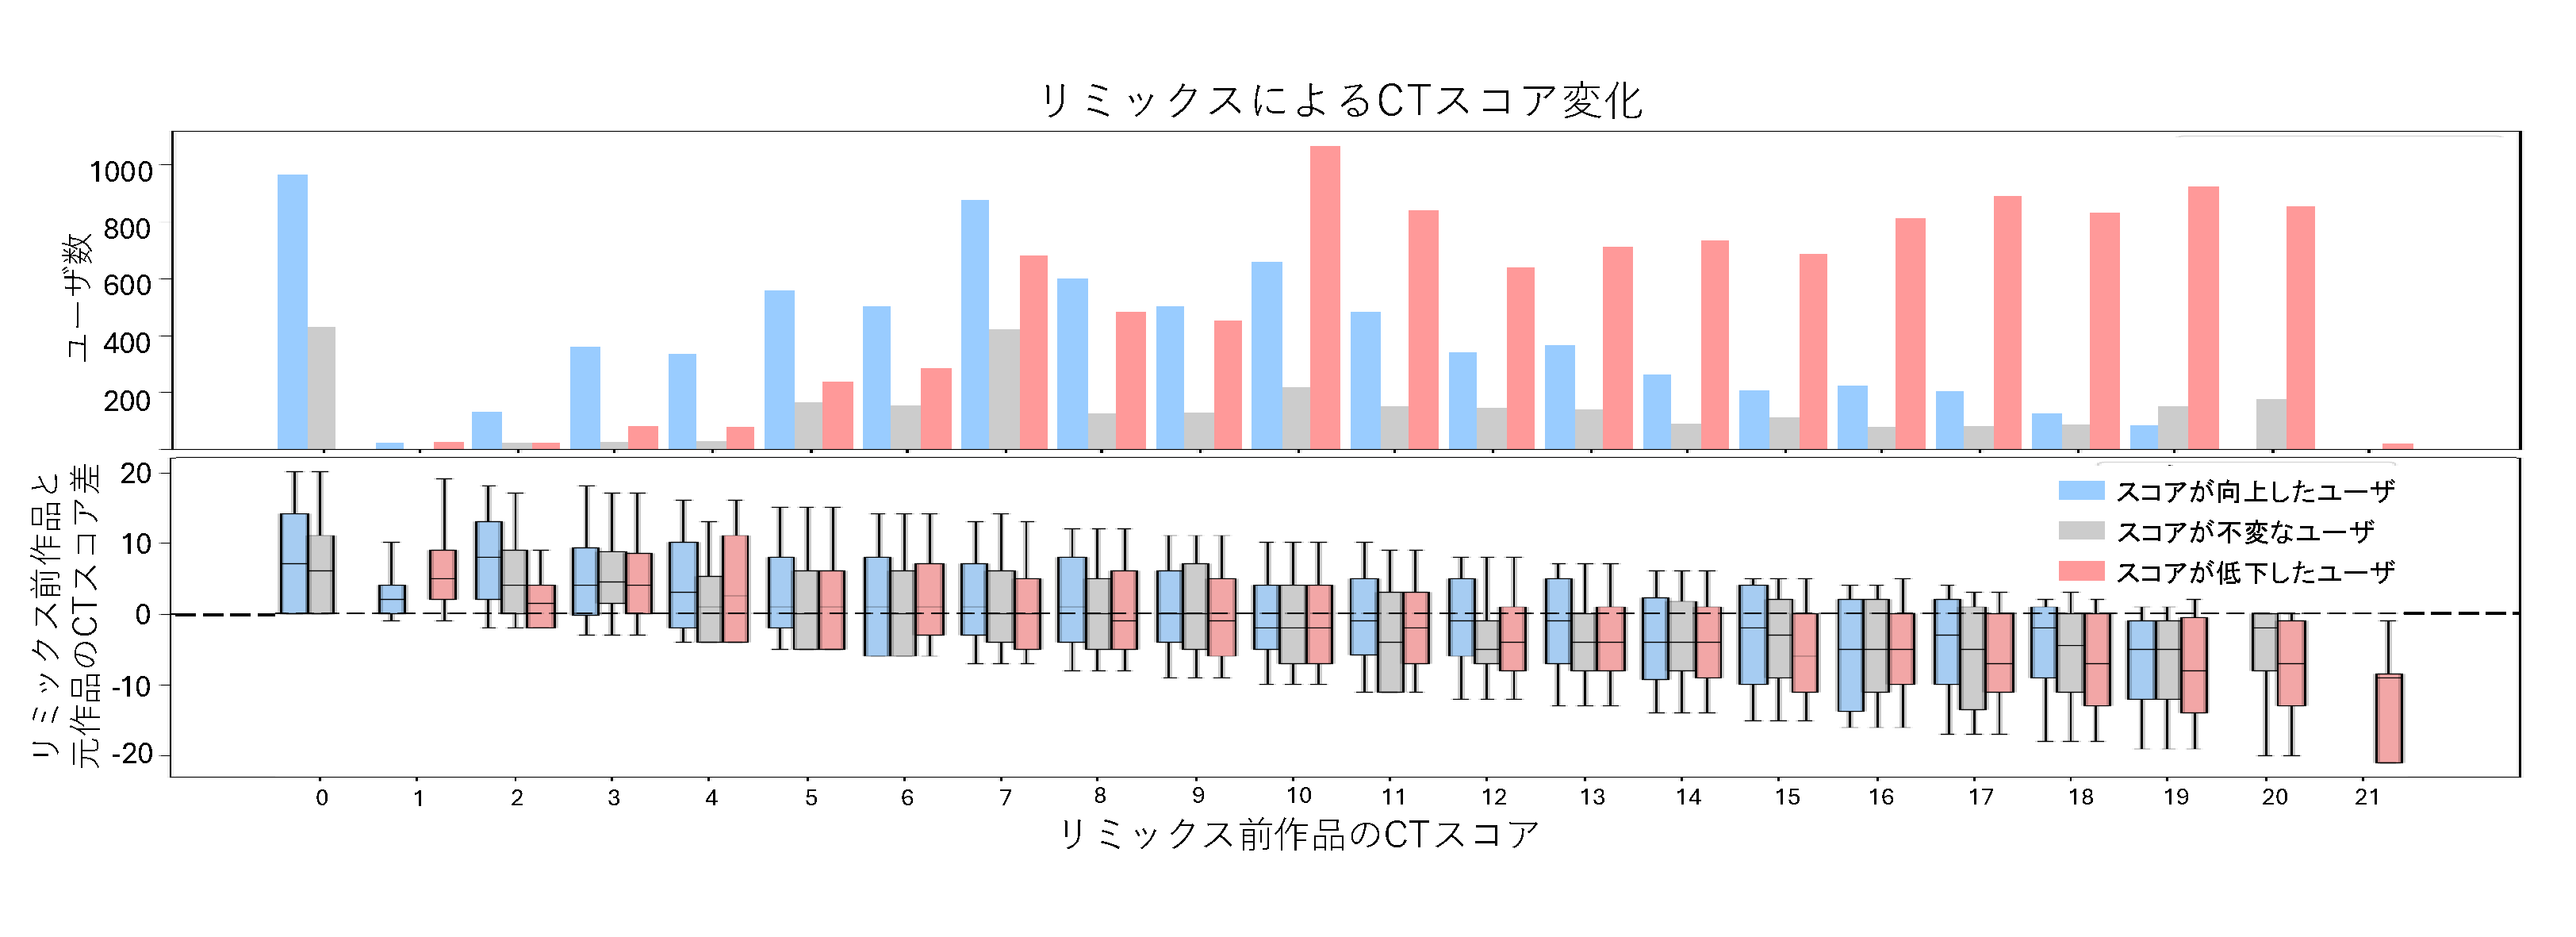
\includegraphics[width=\textwidth]{@IPSJ_SIGSE202511_Horio/fig/preAnalysis.pdf}
  \caption{ユーザの熟練度とリミックス元作品のCTスコアの関係}
  \label{preAnalysis}
\end{figure*}
%----------------------
\begin{figure}[h]
  \centering
  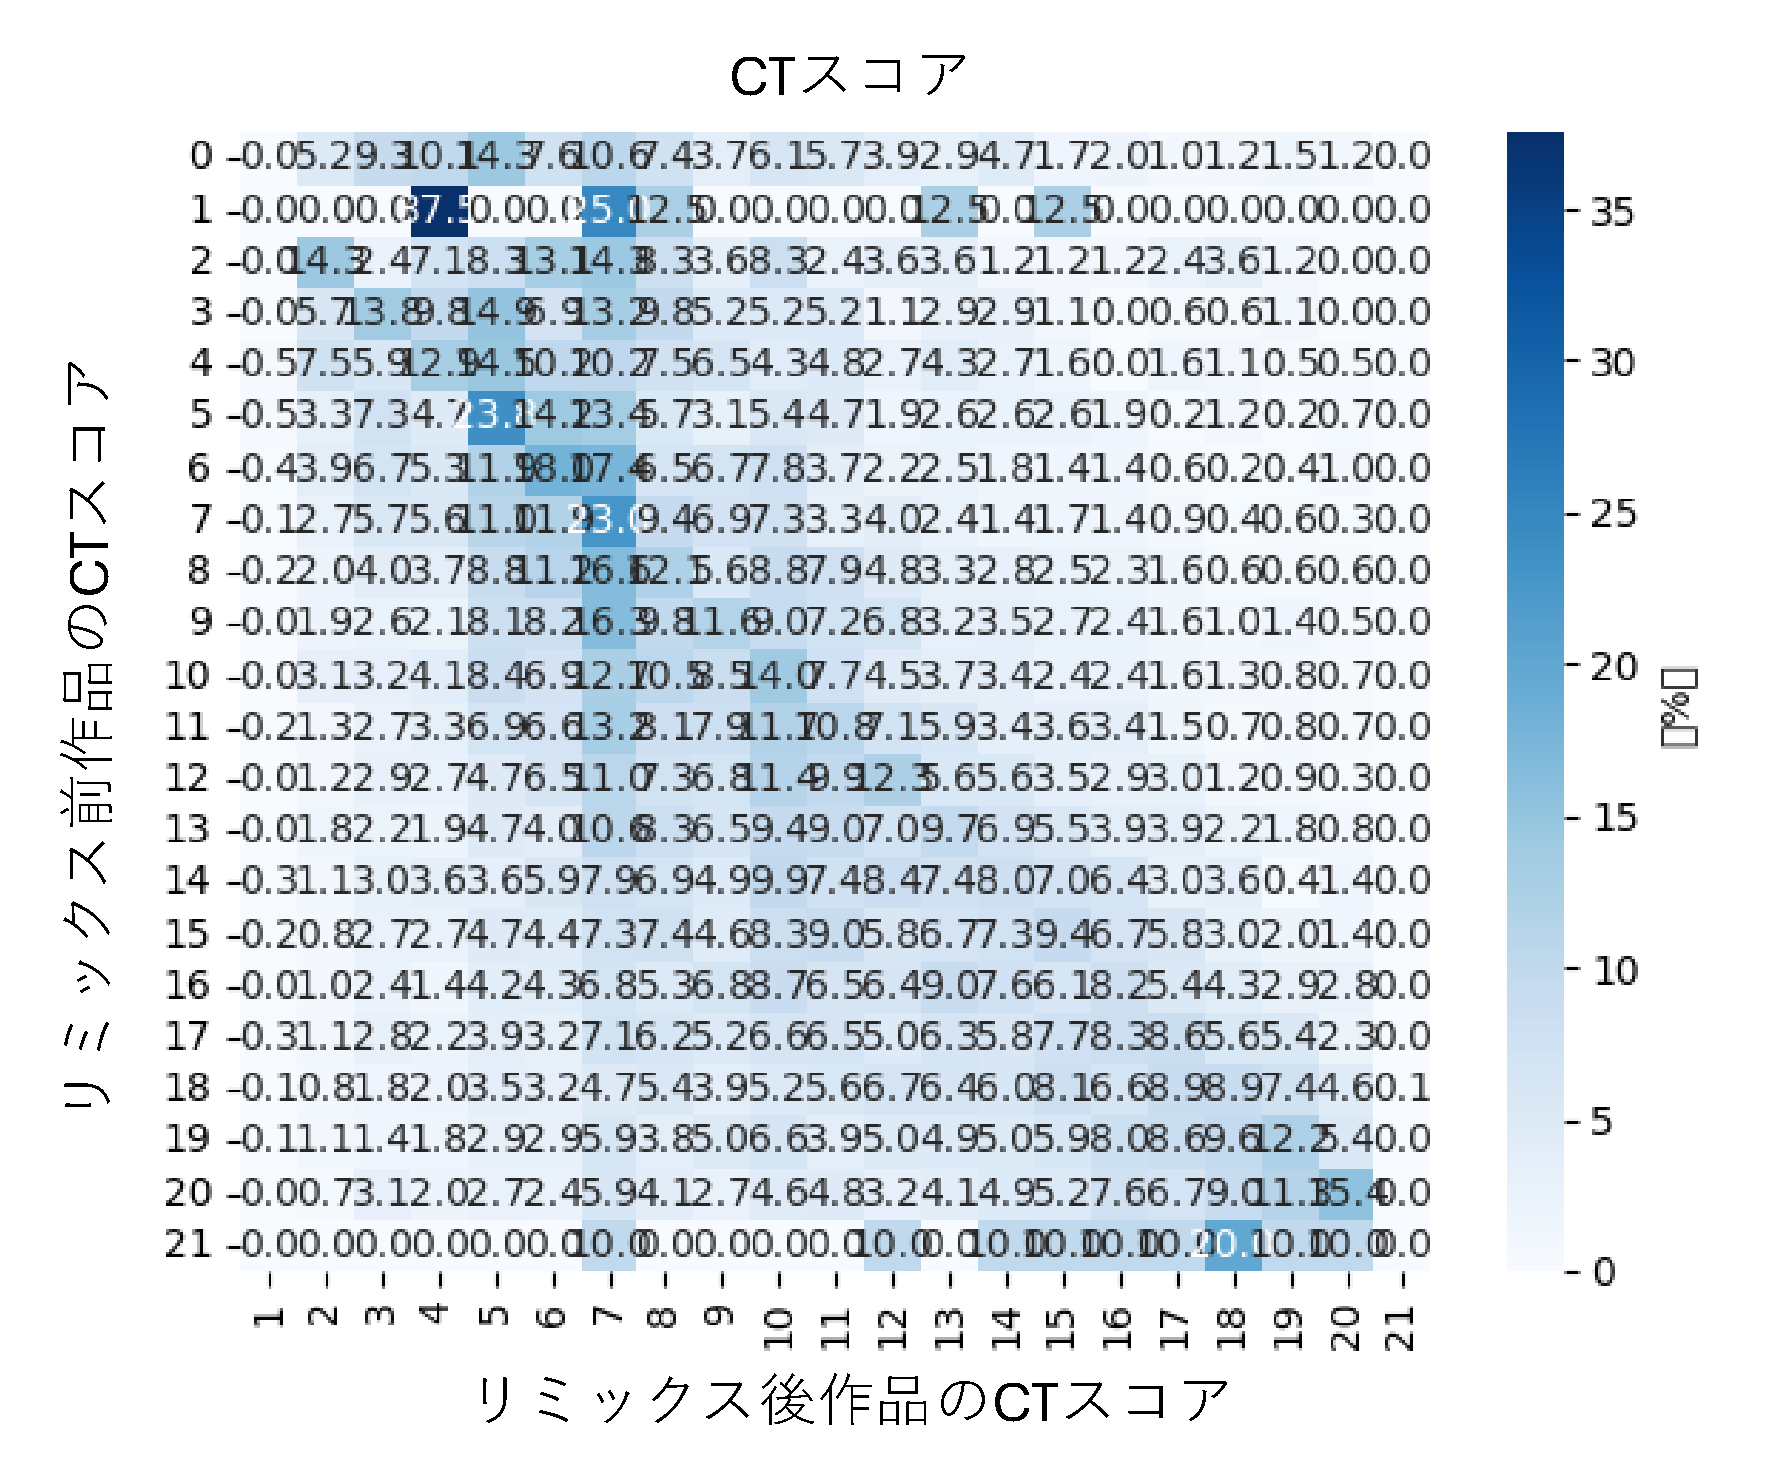
\includegraphics[width=\linewidth]{@IPSJ_SIGSE202511_Horio/fig/heatmapCT.pdf}
  \caption{CTスコアのヒートマップ}
  \label{heatmapCT}
\end{figure}

%%%%%%%%%%%%%%%%%%%%%%%%%%%
\section{用語の定義}
\label{sec:preAnalysis}
%%%%%%%%%%%%%%%%%%%%%%%%%%%

本研究では,ユーザがリミックスによって制作した作品,およびその前後の作品を分析対象として分析を進める.本章では,分析で取り扱うデータセットで使用する用語の定義を説明する.図\ref{teigi}は,分析で取り扱うデータセットの概略図を示す.

\begin{figure*}[t]
  \centering
  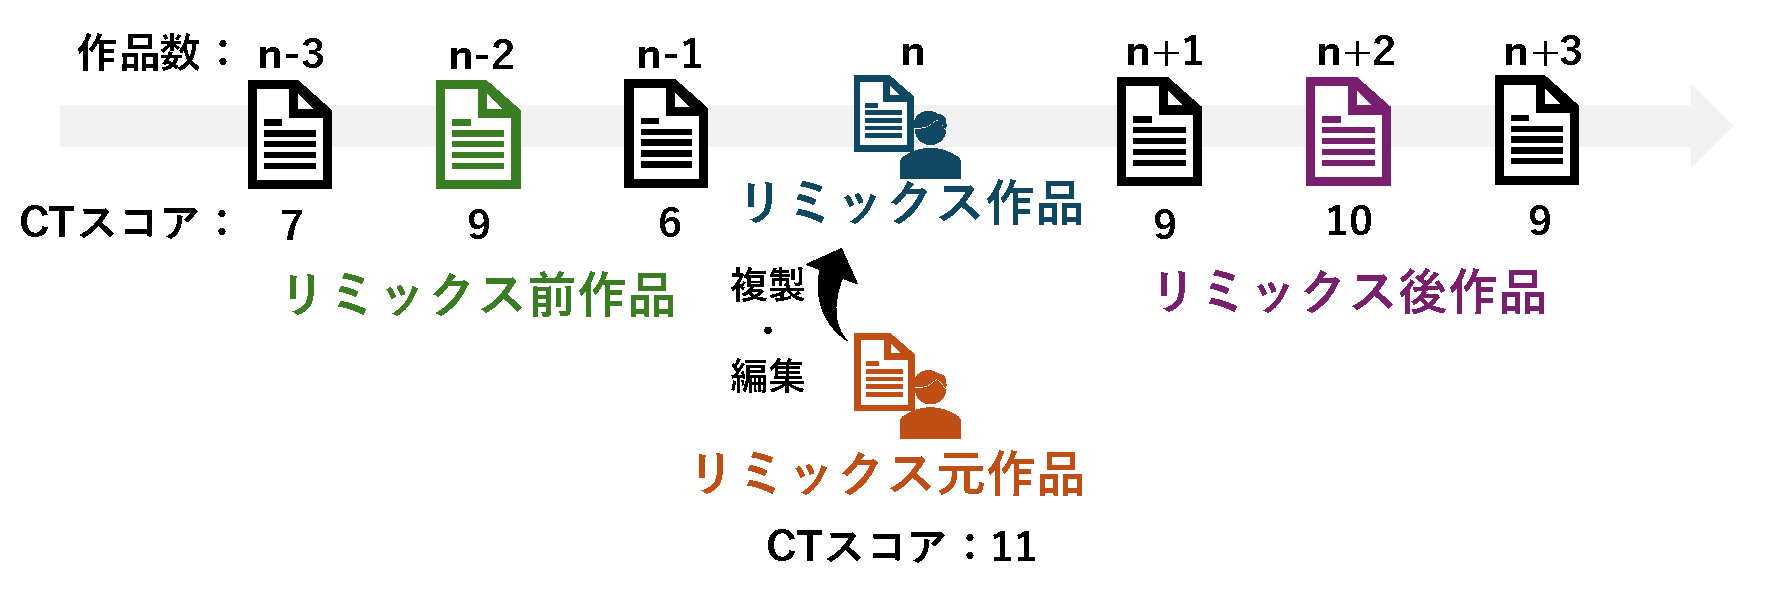
\includegraphics[width=0.7\linewidth]{@IPSJ_SIGSE202511_Horio/fig/teigi.pdf}
  \caption{本研究における用語の定義}
  \label{teigi}
\end{figure*}

\begin{itemize}
    \item オリジナル作品
  
    ユーザがリミックスの機能を使用せずに制作した作品.

    \item リミックス作品

    ユーザがリミックスによって制作した作品とする.ユーザが制作した20作品のうち,複数の作品がリミックスによって制作されている場合は,それらすべてを対象に含める.ただし,リミックスによって制作された作品が連続している場合には,どの作品をリミックスしたことによる効果であるかを区別できないため,連続するリミックス作品はいずれも分析対象から除外する.
     
    \item リミックス元作品

    Scratchが公開する作品の中で,ユーザがリミックスに使用する作品とする.
    
    \item リミックス前作品
  
    リミックス作品の直前に制作した3作品がすべてオリジナル作品の中で,獲得したCTスコアが最も高い作品とする.また,その作品のCTスコアをユーザのリミックス時点における熟練度とする.

    \item リミックス後作品
  
    リミックス作品の直前に制作した3作品がすべてオリジナル作品の中で,獲得したCTスコアが最も高い作品とする.また,その作品とリミックス前作品のCTスコアを比較した差分をリミックスによる効果とする.3件以下とした理由は,オリジナル作品の制作を重ねることによるCTスコア向上の影響を軽減するためである.
\end{itemize}



%%%%%%%%%%%%%%%%%%%%%%%%%%%
\section{RQ1:ユーザの熟練度によってリミックスの影響は異なるか?}
\label{sec:rq1}
%%%%%%%%%%%%%%%%%%%%%%%%%%%

従来研究\cite{10.1145/2724660.2724674}\cite{hashitani2022scratch}\cite{10.1145/2818048.2819984}でリミックスによりCTスコアが向上することを示されたが,RQ1では,リミックス後作品のCTスコアが向上するのは,リミックス前作品のCTスコアに応じて異なるか否かを明らかにする.

\subsection{CTスコア合計点の結果}

図\ref{preAnalysis}は,リミックス前作品のCTスコア(熟練度)と,リミックス作品のCTスコアとの違いを示すことで,ユーザがリミックスのために選択する作品の特徴を明らかにする.青色は,リミックス前作品に比べてリミックス後作品のCTスコアが向上したユーザ,灰色はCTスコアに変化のないユーザ,赤色はCTスコアが低下したユーザを示す.特に,図\ref{preAnalysis}上図は,熟練度別のユーザ数を棒グラフで示し,図\ref{preAnalysis}下図は,ユーザの熟練度においてリミックス元作品のCTスコア差を箱ひげ図で示す.

% 分析の結果を図\ref{preAnalysis},図\ref{preAnalysis2}に示す.図\ref{preAnalysis}はリミックス前後作品のCTスコア変化の箱ひげ図と分布グラフであり,リミックス前作品に比べてリミックス後作品のCTスコアが向上したユーザが青色,不変なユーザが灰色,低下したユーザが青色である.

リミックス前作品のCTスコアが9点以下のユーザは,図\ref{preAnalysis}上図より,リミックス後作品でCTスコアが向上しているユーザが多い.特に図\ref{preAnalysis}下図より,その点よりも高いCTスコアの作品をリミックスしていることが多い.

リミックス前作品のCTスコアが10点以上のユーザは,図\ref{preAnalysis}上図より,リミックス後作品でCTスコアが低下しているユーザが多い.特に図\ref{preAnalysis}下図より,その点よりも低いCTスコアの作品をリミックスしていることが多い.

図\ref{heatmapCT}は,これらの結果を詳細に調査した結果を示す.横軸にリミックス後作品のスコア,縦軸にリミックス前作品のスコアを配置し,各セルにはリミックス前作品のCTスコアに基づいた分布率を示す.リミックス前作品のスコアデータの偏りによる影響を抑えるため,リミックス前作品のスコアを基準として相対的に値を算出する.分析の結果,リミックス前作品のCTスコアが9点前後から,スコアが低下しているユーザの割合が増加してくる.また,リミックス前作品のCTスコアが8点以上ではリミックス後作品のCTスコアが7点に低下しているユーザと不変のユーザの分布が同じくらいになっている.加えて,リミックス前作品のCTスコアが7点以下のユーザは約3,4点向上している.


% スコアが向上したユーザ数が低下したユーザ数を上回っているが,10点以上はスコアが低下したユーザ数が向上したユーザ数を上回っている.また,スコアが向上している多くのユーザは自身のCTスコアよりも高い作品をリミックス元作品として選択している.\memo{低下しているユーザよりも高い作品?}これらのことから,初級者はリミックスによる効果を得やすいこと,自身のCTスコアより高い作品のリミックスが有効であることが示唆される.

% 詳細をヒートマップで示す.
% 分析手法としてヒートマップを用いる.

% CTスコアの結果は図\ref{heatmapCT},

% CTスコアの

\subsection{概念別CTスコアの結果}

図\ref{preAnalysis2}は,図\ref{preAnalysis}と同様に棒グラフと箱ひげ図で,リミックス前作品のCTスコア(熟練度)と,リミックス作品のCTスコアとの違いを概念別に示す.
% CTスコアの各概念スコア変化の箱ひげ図と分布グラフである.縦軸をリミックス前作品とリミックス元作品のスコア差とすることで,ユーザが自身の熟練度に対し,どのスコアの作品を選択し,リミックスしているのかわかる.

% \todo{この段落はCTスコアと同じことを概念別と言ってるだけなので,スペース次第では優先的に削除しても良い.}図\ref{preAnalysis2}は,概念別にリミックス前作品のCTスコア(熟練度)と,リミックス作品のCTスコアとの違いを示すことで,ユーザがリミックスのために選択する作品の概念別のCTスコアの特徴を明らかにする.青色は,リミックス前作品に比べてリミックス後作品のCTスコアが向上したユーザ,灰色はCTスコアに変化のないユーザ,赤色はCTスコアが低下したユーザを示す.特に,図\ref{preAnalysis2}上図は,概念ごとに熟練度別のユーザ数を棒グラフで示し,図\ref{preAnalysis2}下図は,ユーザの熟練度においてリミックス元作品のCTスコアとのスコア差を箱ひげ図で示す.


% リミックス前作品のCTスコアが9点以下のユーザは,図\ref{preAnalysis}上図より,リミックス後作品でCTスコアが向上しているユーザが多い.特に図\ref{preAnalysis}下図より,その点よりも高いCTスコアの作品をリミックスしていることが多い.

抽象化と論理はリミックス前作品のCTスコアが0点,その他の概念は1点以下のユーザに関して,図\ref{preAnalysis2}上図より,リミックス後作品でCTスコアが向上しているユーザが多い.したがって,抽象化と論理はリミックスすることで使い方を学び,その他の概念はブロックの応用方法をリミックスすることで学んでいることが示唆される.

% リミックス前作品のCT各概念のスコアが2点の地点では,スコアが向上したユーザ数が低下したユーザ数に比べて非常に少ない.しかし,スコアが向上しているユーザも見られることから,ユーザの熟練度に適した作品をリミックスすると,スコアが向上する可能性が考えられる.また,スコアが向上しているユーザは低下しているユーザに比べ,スコアが高い作品をリミックスしている場合が多い.
% このことから,ユーザのCT各概念スコアを考慮し,推薦する必要性が示唆される.
% \memo{だからスコアが向上しているユーザから学習して,推薦が必要になると思ってる}


図\ref{heatmap}は,これらの結果を概念別に詳細に調査した結果を示す.図\ref{heatmapCT}と同様に,横軸にリミックス後作品のスコア,縦軸にリミックス前作品のスコアを配置し,各セルにはリミックス前作品のスコアに基づいた分布率を示す.

データ表現やユーザ対話性,フロー制御,抽象化はリミックス前作品のスコアが0点のユーザがリミックス後作品でスコアが向上しているユーザが多く,特にユーザ対話性,フロー制御では0点から2点に向上しているユーザが多い.したがって,この4概念が0点のユーザはリミックスによって学んでいることが示唆される.

並列処理はリミックス後作品のスコアが1点のユーザが多く,また,リミックス前作品のスコアが0点では,リミックス後作品のスコアが0点のままであるユーザが多い.
同期では,リミックス前作品とリミックス後作品のスコアが同等のユーザが多く,また,論理ではリミックス後作品のスコアが0点のユーザが多い.したがって,並列処理や同期,論理ではリミックスによりスコアが向上し難い可能性がある.

% CT各概念においてリミックス前作品のスコアが0点で,リミックスが効果的であるものとして,データ表現,ユーザ対話性,フロー制御,抽象化があげられる.

% CT各概念は,リミックスによってスコアが向上しやすい概念,変動し難い概念,低下しやすい概念の3種類に分類できる.

% 向上しやすい概念として,ユーザ対話性,フロー制御が挙げられる.リミックス前作品で0点のユーザが1,2点に向上しているユーザの割合が多い.

% 変動し難い概念として,同期が挙げられる.リミックス前作品のスコアとリミックス後作品のスコアが同等のユーザの割合が多い.

% 低下しやすい概念として,データ表現,並列処理,抽象化,論理が挙げられる.いずれもリミックス前作品で2点,3点を取得しているユーザがリミックス後作品に低下しているユーザが多い.しかし,維持することができているユーザや向上しているユーザもみられる.


% \color{red}
% データ表現では,リミックス前作品のスコアが0点,1点のユーザはリミックス後作品のスコアが1点のユーザの割合が多く,リミックス前作品のスコアが2点ではリミックス後作品のスコアが1点,2点のユーザの割合が多くなっている.また,リミックス前作品のスコアが3点では1から3点に均等に分布している.
% ユーザ対話性では,リミックス後作品のスコアが1点,2点に分布が集中している.
% 並列処理では,リミックス後作品のスコアが2点のユーザの割合が非常に少ない.また,リミックス前作品のスコアが3点のユーザはスコアを維持しているユーザが多い.
% フロー制御では,リミックス後作品のスコアが2点に分布が集中している.また,リミックス前作品のスコアが3点のユーザはスコアを維持しているユーザも多く存在する.
% 抽象化では,リミックス後作品のスコアが1点のユーザが多く,2点のユーザの割合が少ない.また,リミックス前作品のスコアが3点のユーザはスコアを維持している場合も多く存在する.
% 同期では,基本的にはどのスコアでも不変なユーザが多いが,リミックス前作品が1点のユーザが0点に,3点のユーザが2点に低下してしまっている場合も多く存在する.
% 論理では,リミックス後作品のスコアが0点のユーザが多く,リミックス前作品のスコアが3点のユーザはスコアを維持している場合も多く存在する.
% \color{black}

% 学習者の熟練度に応じて最適なリミックス元作品が存在することが示唆された.すなわち,学習者の熟練度に応じたリミックス元作品の推薦が学習支援として有効であることが考えられる.


%---------------------
\begin{figure}[t]
  \centering
  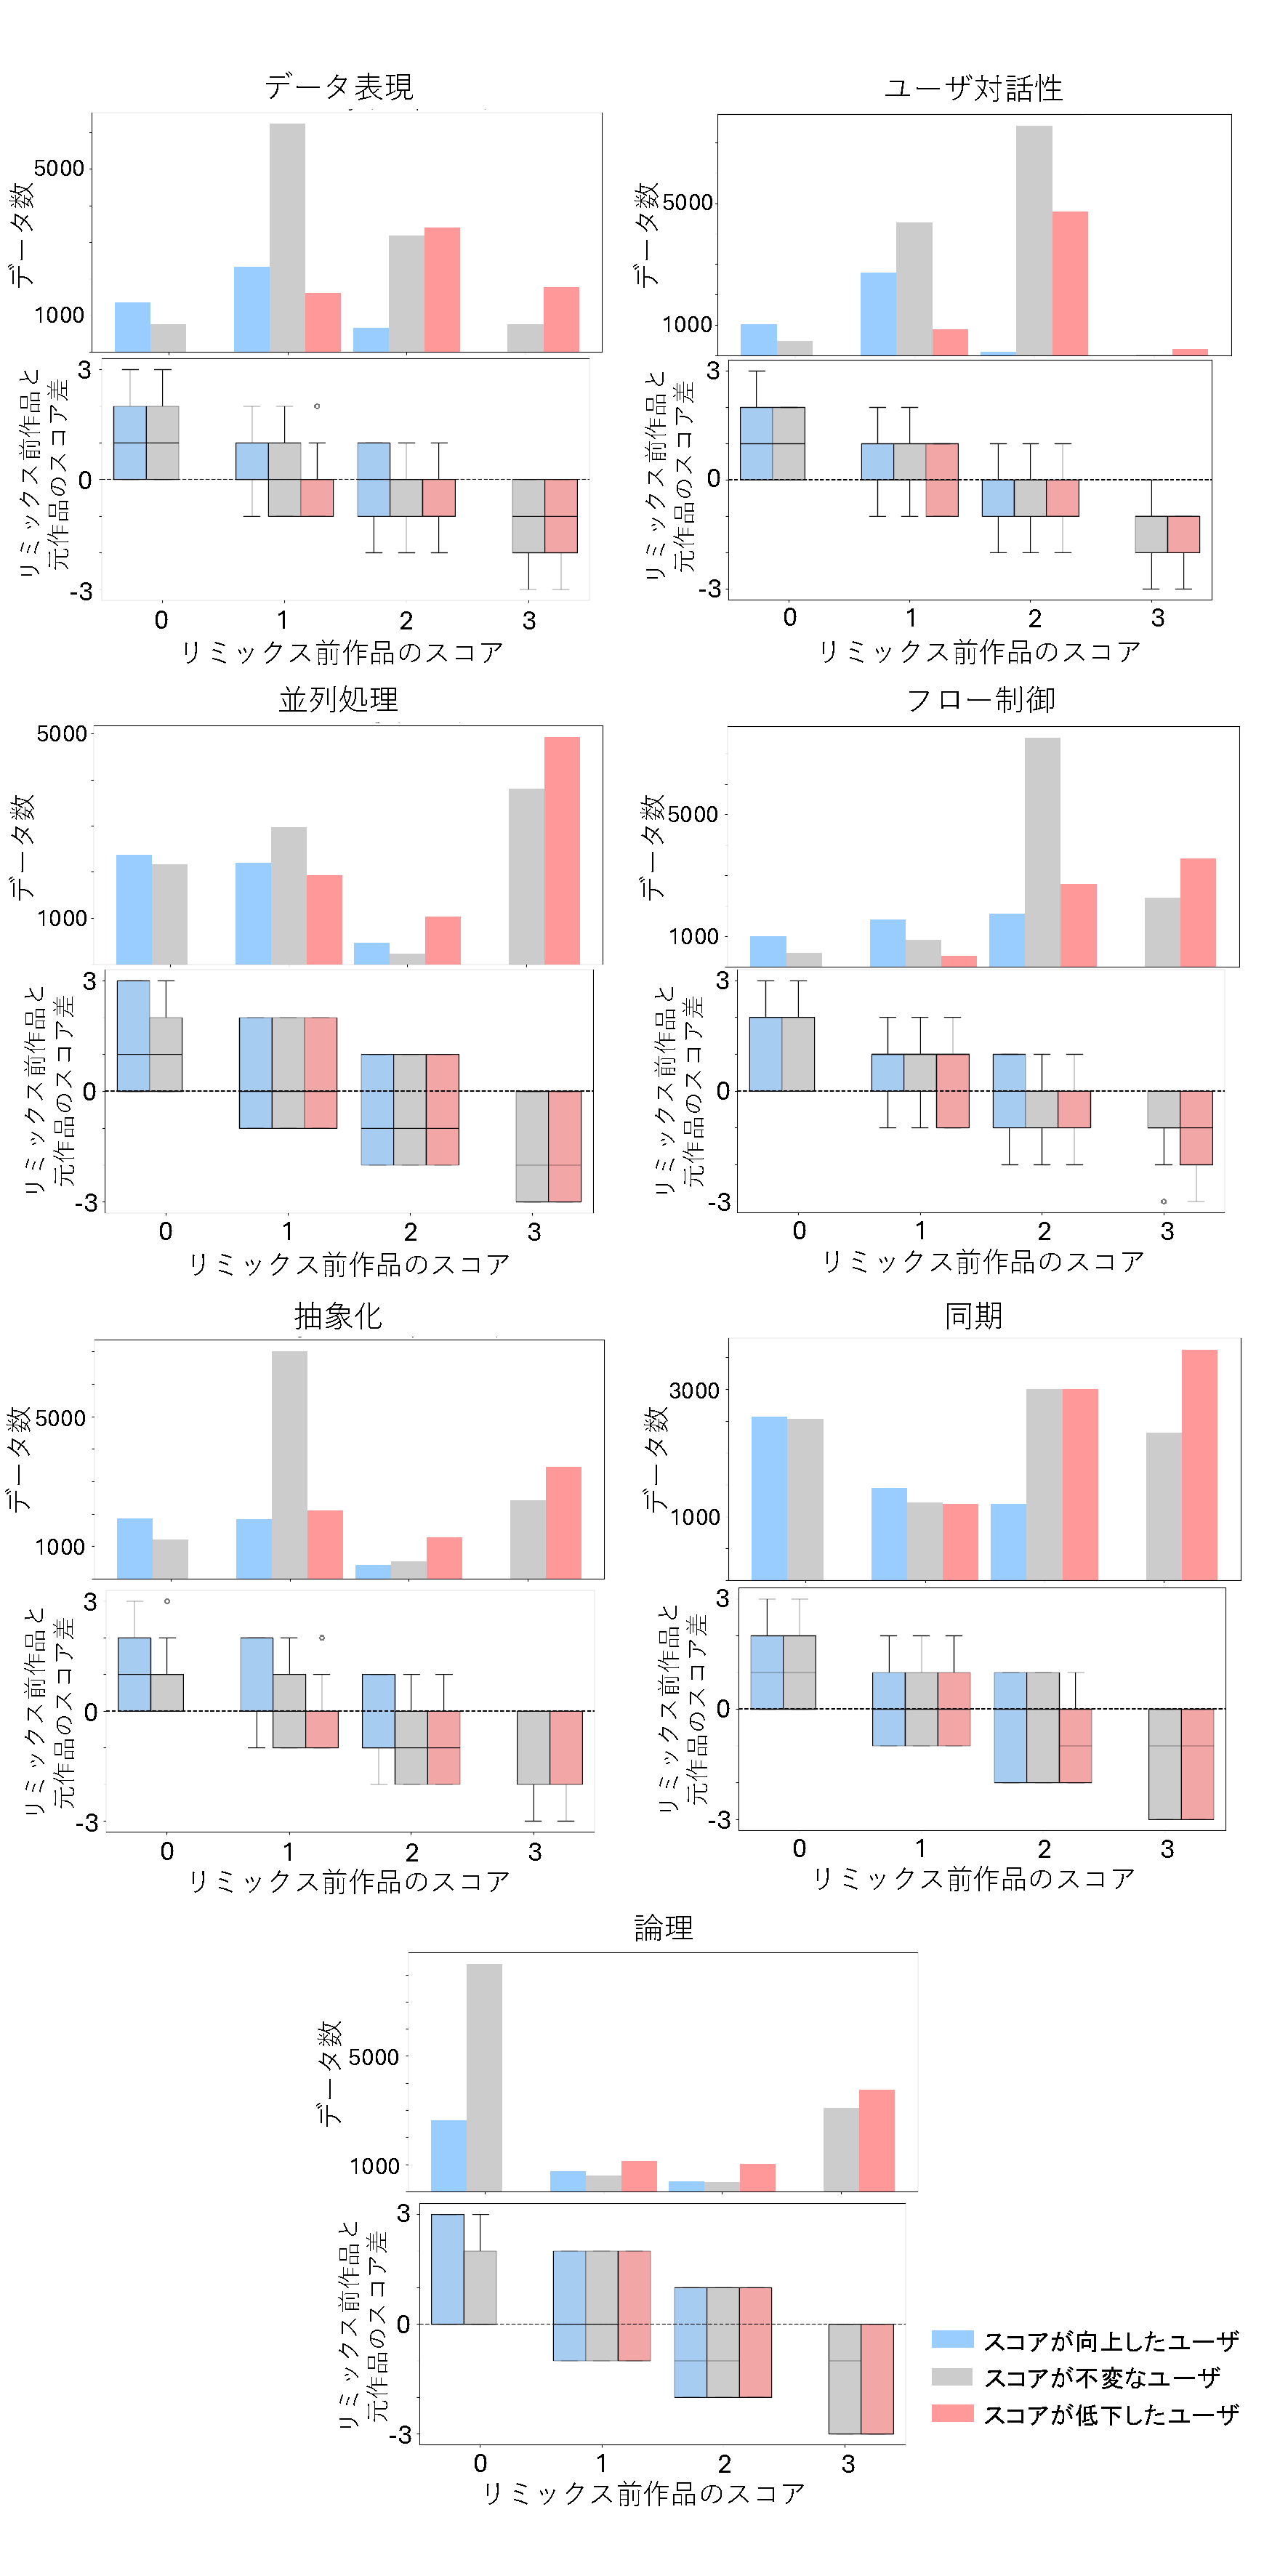
\includegraphics[width=\linewidth]{@IPSJ_SIGSE202511_Horio/fig/preAnalysis2.pdf}
  \caption{ユーザの熟練度とリミックス元作品のCT各概念スコアの関係}
  \label{preAnalysis2}
\end{figure}
%---------------------

%---------------------
\begin{figure*}[t]
  \centering
  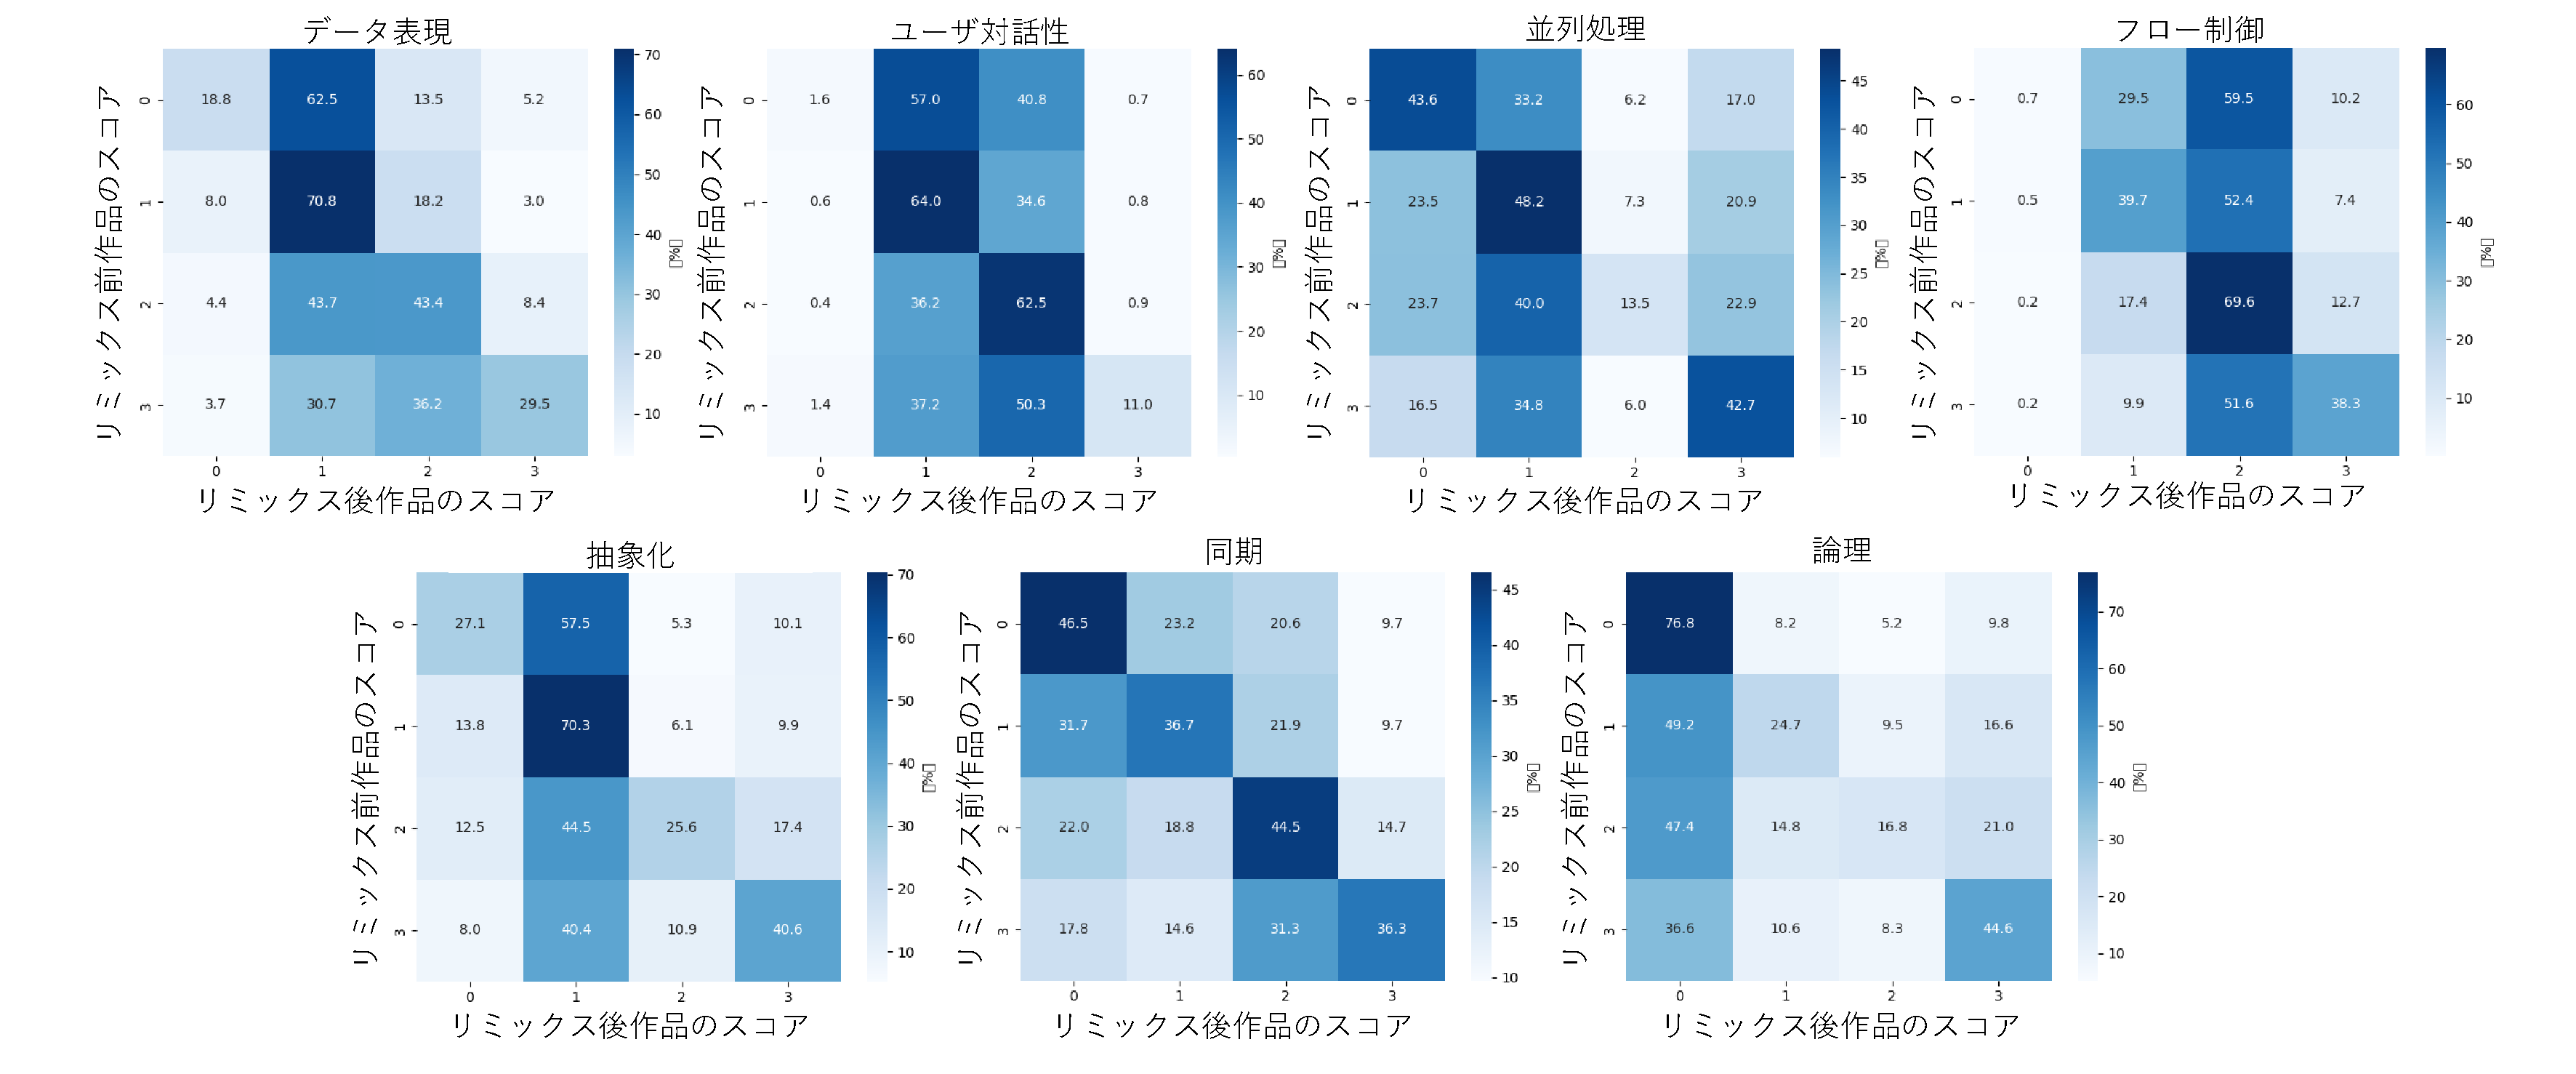
\includegraphics[width=\textwidth]{@IPSJ_SIGSE202511_Horio/fig/heatmapCTf.pdf}
  \caption{CT各概念のヒートマップ}
  \label{heatmap}
\end{figure*}
%---------------------

% CT概念ごとの結果は図\ref{heatmap}に示す.
% CTスコアの結果では,リミックス前作品のCTスコアが7点以下のユーザはリミックスを経ることで,CTスコアが低下しているユーザより向上しているユーザの割合が大きくなっている.しかし,リミックス前作品のCTスコアが8点以上のユーザはリミックスを経ても,CTスコアが向上しているユーザより低下しているユーザの割合が大きくなっている.そのため,リミックスはCTスコアが7点以下のユーザに特に効果が現れやすいことがわかる.



% CT各概念の結果では,リミックスによってスコアが向上しやすい概念と変動し難い概念,低下しやすい概念に分かれている.

% データ表現では,リミックス前作品のスコアが0点,1点のユーザはリミックス後作品のスコアが1点のユーザの割合が多く,リミックス前作品のスコアが2点ではリミックス後作品のスコアが1点,2点のユーザの割合が多くなっている.また,リミックス前作品のスコアが3点では1から3点に均等に分布している.
% ユーザ対話性では,リミックス後作品のスコアが1点,2点に分布が集中している.
% 並列処理では,リミックス後作品のスコアが2点のユーザの割合が非常に少ない.また,リミックス前作品のスコアが3点のユーザはスコアを維持しているユーザが多い.
% フロー制御では,リミックス後作品のスコアが2点に分布が集中している.また,リミックス前作品のスコアが3点のユーザはスコアを維持しているユーザも多く存在する.
% 抽象化では,リミックス後作品のスコアが1点のユーザが多く,2点のユーザの割合が少ない.また,リミックス前作品のスコアが3点のユーザはスコアを維持している場合も多く存在する.
% 同期では,基本的にはどのスコアでも不変なユーザが多いが,リミックス前作品が1点のユーザが0点に,3点のユーザが2点に低下してしまっている場合も多く存在する.
% 論理では,リミックス後作品のスコアが0点のユーザが多く,リミックス前作品のスコアが3点のユーザはスコアを維持している場合も多く存在する.


\subsection{考察}

CTスコアについて,8点付近から向上させることが難しく,学習支援の必要性が示唆される.

CT概念の結果について,表\ref{CTscoreTable}の内容と照らし合わせながら結果を考察する.

まず,データ表現,ユーザ対話性,フロー制御,抽象化について考察を行う.作品内に画像オブジェクトなどを使用し,動かす場合にはデータ表現が1点になる.これはScratchのチュートリアル序盤でも学習可能な内容であり,基礎部分にあたるため,多くのユーザが実装しやすいと考えられる.
ユーザ対話性について,緑の旗ブロックを使用すると1点となり,これは作品を動かす上で必須となっているため多く存在すると考えられる.また,2点はキーボード入力などを必要とするものであり,ゲームなどで利用されやすい.しかし,3点ではマイクやビデオなどの作用が必要であり,利用者の動作環境が必ず整っているわけでないことから,実装不要の可能性も示唆される.
フロー制御について,結果を見ると低下したユーザの割合は少なくなっている.これはテキストプログラミングの学習と同じで,繰り返しブロックの実装方法を知ることで,何度も同じコードを書く必要がなくなる.そのため,2点,3点取得後は繰り返しブロックを積極的に利用する傾向にあると考える.
抽象化について,2点の項目である定義ブロックは自身でブロックを作成することであり,必要最低限のブロックが多く用意されているScratchではあまり利用することがないブロックであることが考えられる.

次に,並列処理,同期,論理について考察を行う.並列処理では,リミックス後作品のスコアが2点のユーザが極端に少なくなっているが,その原因として考えられるのは,3点の実装内容の影響である.3点の実装方法を学習することで,2点の実装方法でプログラムする必要がなくなってしまう.
同期について,あまり変動がなく,リミックスにより効果を得難い可能性がある.また,リミックス前作品のスコアが3点のユーザが2点に低下している場合がみられる.これは,3点の実装方法を習得済みであるが,実装したい内容がメッセージ受信によるものであることから2点の実装方法を利用している可能性がある.
論理についてはifブロック,if elseブロックの実装場面がそもそも少ない可能性が考えられ,また,リミックスによる効果も得難い可能性が考えられる.

これらの結果からリミックスによる学習効果は一様ではなく,スコアが向上しやすいCT概念もあれば,向上し難いCT概念もある.また,スコアが向上しているユーザもいれば,低下しているユーザも多く存在する.したがって,スコアが向上しているユーザのCT概念のスコア,リミックス元作品の選択をもとに,リミックス対象作品を予測する本研究のモデルが有用であることが示唆される.また,初級者はリミックスをすると比較的スコアが向上しやすく,中級者あたりからスコアが向上しづらくなる.このことから熟練度によってモデルを分類する必要性も示唆される.

% これらの結果からリミックスによる学習効果は一様ではなく,ユーザのリミックス前作品のCTスコア合計点が9点未満の初学者は,リミックスによりCTスキルが向上することが多いことを明らかにした.したがって,本研究が提案するリミックス対象作品のCTスコアを予測するモデルは,Scratch初学者のユーザに有用であることが示唆される.\todo{一旦こんな感じで.また修正する可能性あり}


% \ihara{ここまで修正済み}

%%%%%%%%%%%%%%%%%%%%%%%%%%%
\section{RQ2:強化学習によるモデルはリミックス元作品のCTスコアを予測できるか?}
\label{sec:rq2}
%%%%%%%%%%%%%%%%%%%%%%%%%%%

本研究では,Scratchユーザがこれから制作する作品が,過去に制作した作品のCTスコアを上回ることに寄与する,リミックス対象作品のCTスコアを予測するモデルを構築する.具体的には,作品の制作過程をマルコフ決定過程として捉え,強化学習を用いてユーザの学習経験に応じてリミックスした元の作品のCTスコアを予測するモデルを構築する.

\subsection{手法}
強化学習は,機械学習の1つであり,エージェントと呼ばれるシステムが環境と相互作用しながら,試行錯誤を繰り返して,報酬を最大化するような最適な行動(方策)を自律的に学習する手法である.強化学習は主に,エージェント,環境,状態,行動,報酬,方策の要素で構成されている.

ユーザが作品制作した過程をマルコフ決定過程として捉え,強化学習を用いてユーザのリミックス後作品のCTスコアが向上するリミックス元作品を予測するモデルを構築するために,以下のように定義する.

\begin{itemize}
    \item 状態
        
        $s_t$:ある作品制作地点での状態(8次元)\\
        $x_t$:ある作品のCT概念のベクトル(7次元)\\
        $m_t\in\{0,1\}$:リミックスであるか否か(1次元)
        \begin{equation}
            s_t = 
            \begin{bmatrix}
               x_t \\
               m_t 
            \end{bmatrix}
        \end{equation}

    \item 行動

        $a_t$:選択したリミックス元作品のCT概念のベクトル(7次元)

    \item 報酬
    
        $r_t$:リミックス前後作品のCTスコアの差分のスカラー\\
        $c_t$:リミックス前作品のCTスコア\\
        $c'_t$:リミックス後作品のCTスコア
        \begin{equation}
            r_t = c'_t - c_t
        \end{equation}
    
    \item 状態遷移確率
        \begin{equation}
            P(s' \mid s, a)
        \end{equation}

    \item 期待累積報酬

        $Q^{\pi}(s, a)$:期待累積報酬\\
        $\gamma$:割引率\\        
        $\pi$:エージェントが従う方策
        \begin{equation}
            Q^{\pi}(s, a) = \mathbb{E}_{s' \sim P(\cdot \mid s, a)} 
            \left[ r(s, a) + \gamma \, 
            \mathbb{E}_{a' \sim \pi(\cdot \mid s')} 
            \big[ Q^{\pi}(s', a') \big] \right]
        \end{equation}

\end{itemize}

ユーザの学習過程は連続的なものであるため,強化学習はTwin Delayed DDPG(TD3)を用いる.TD3は連続的な行動空間をもつ環境での性能と安定性を大幅に向上させた深層強化学習の1つである\cite{fujimoto2018addressingfunctionapproximationerror}.

評価方法として,教師あり学習であるランダムフォレスト(RF)を用いて推定平均報酬を比較する.Scikit-learnライブラリを使用し,入力をリミックス前作品のCT概念のベクトル,リミックス元作品のCT概念のベクトル,リミックス前後作品のスコア差分のスカラーとし,RFモデルを構築した.
また,データセットの8割を学習データ,2割をテストデータとして用いる.

\subsection{結果}

\begin{figure}[h]
  \centering
  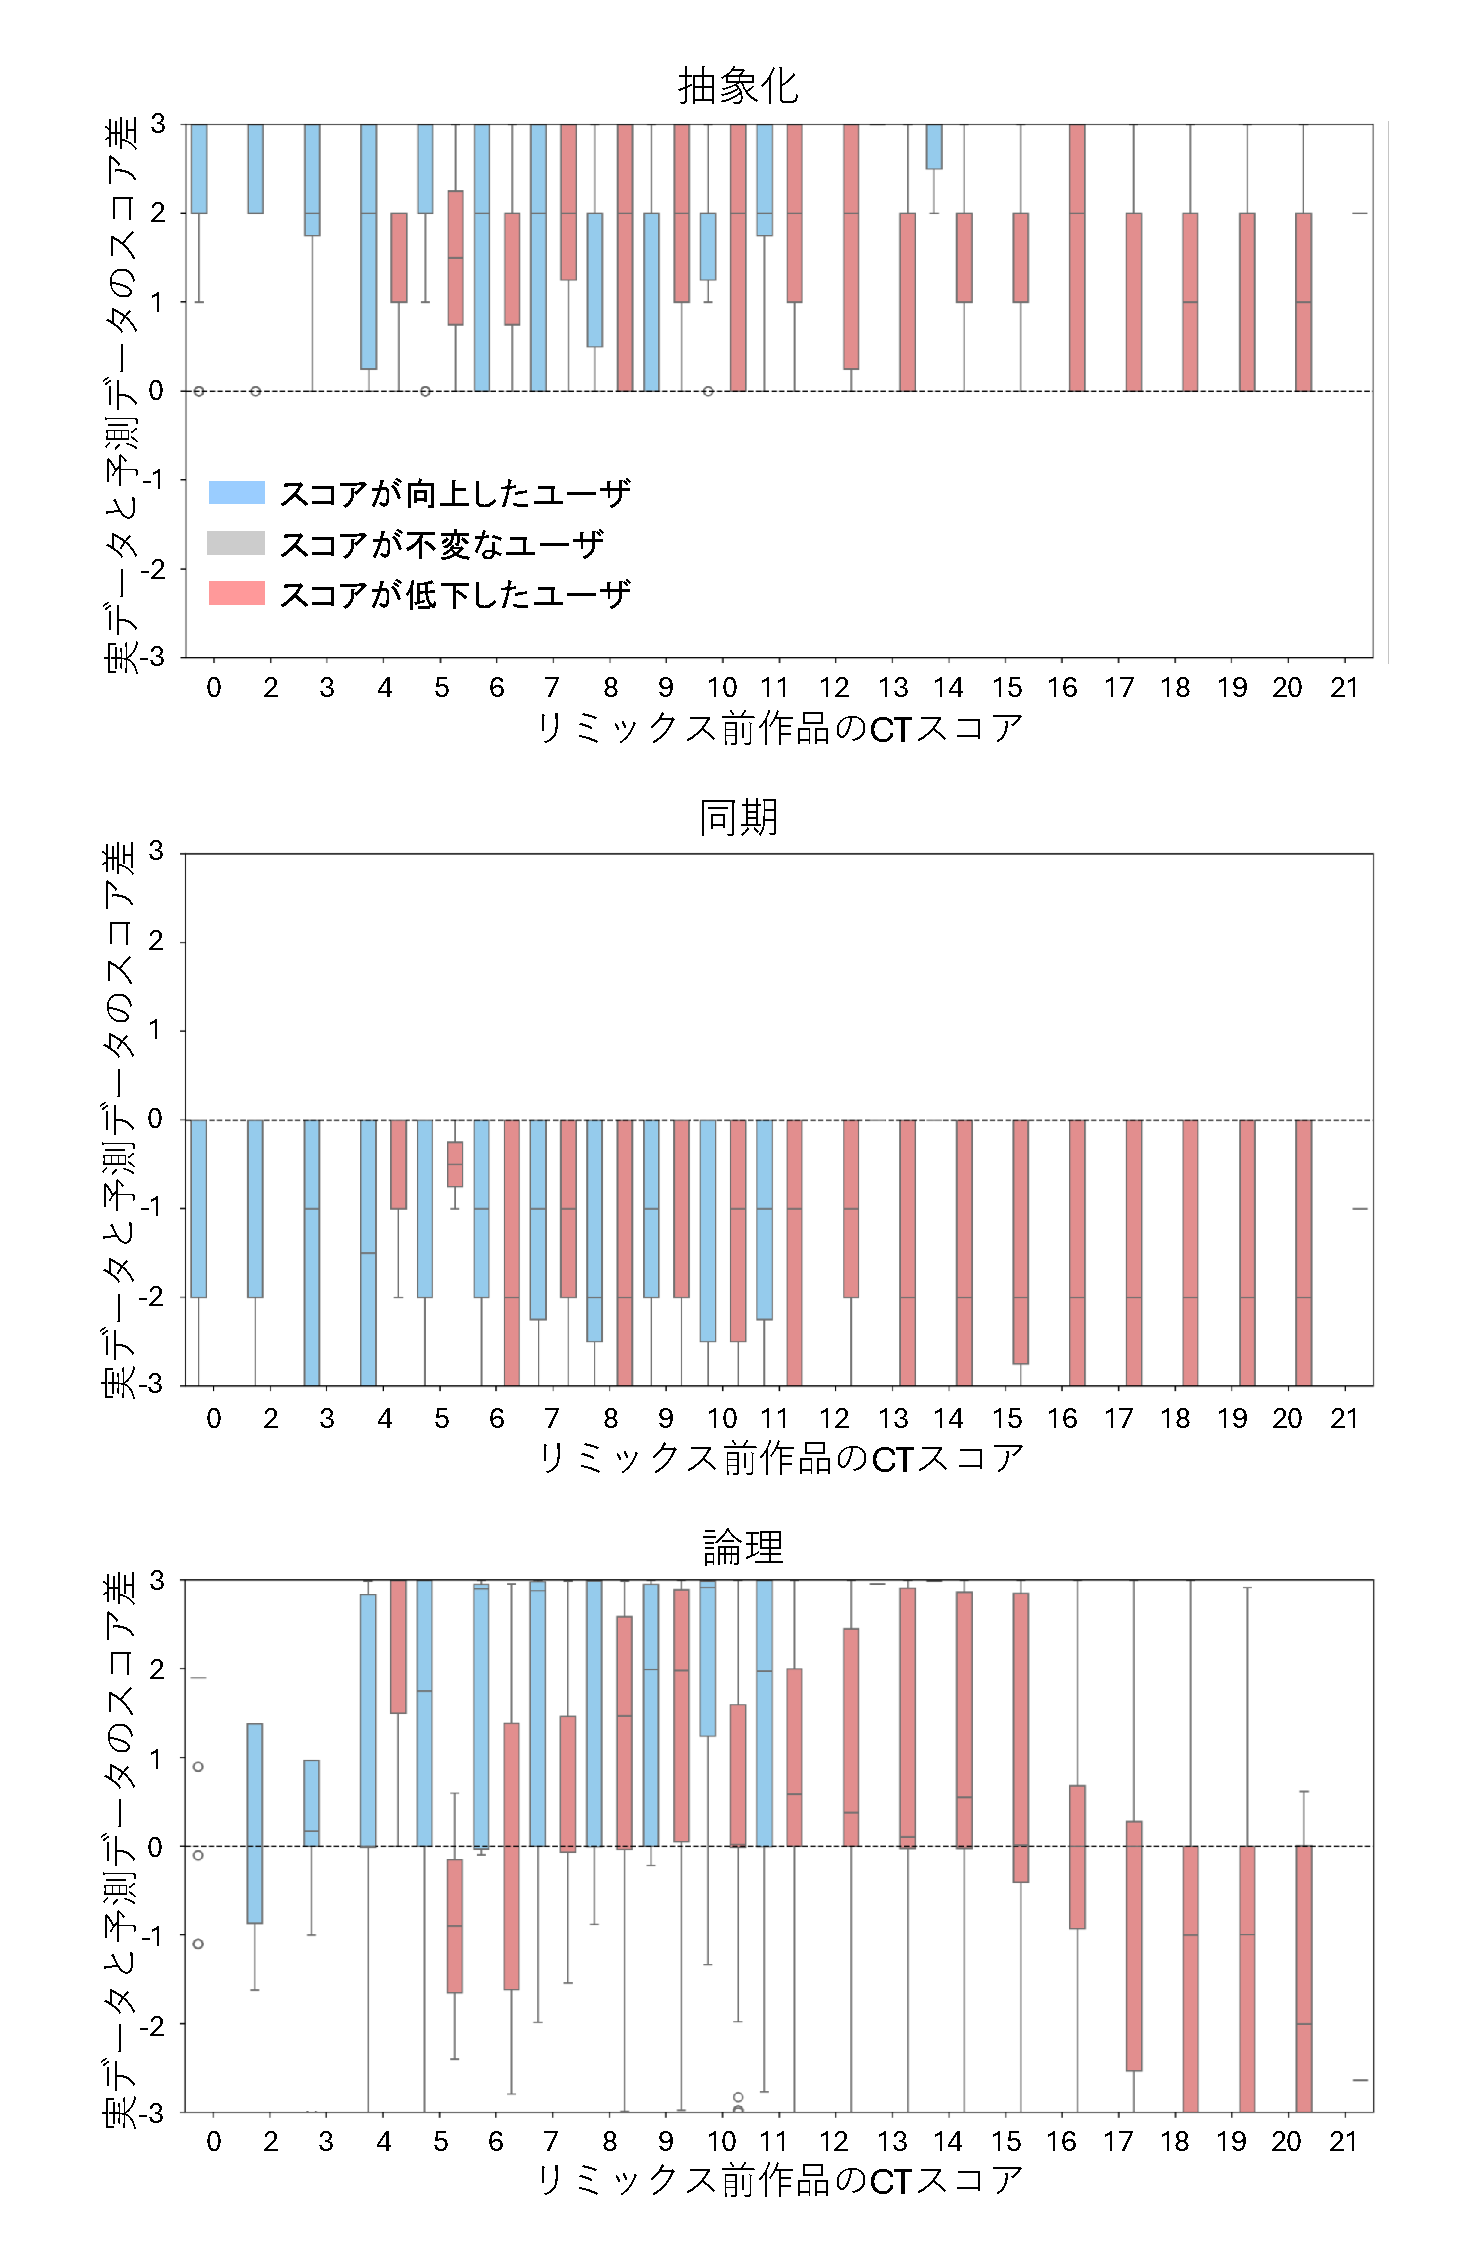
\includegraphics[width=\linewidth]{@IPSJ_SIGSE202511_Horio/fig/diffmini.pdf}
  \caption{実データと予測データのリミックス元作品のCT概念スコア差(一部抜粋)}
  \label{diffminigraph}
\end{figure}

\begin{figure}[h]
  \centering
  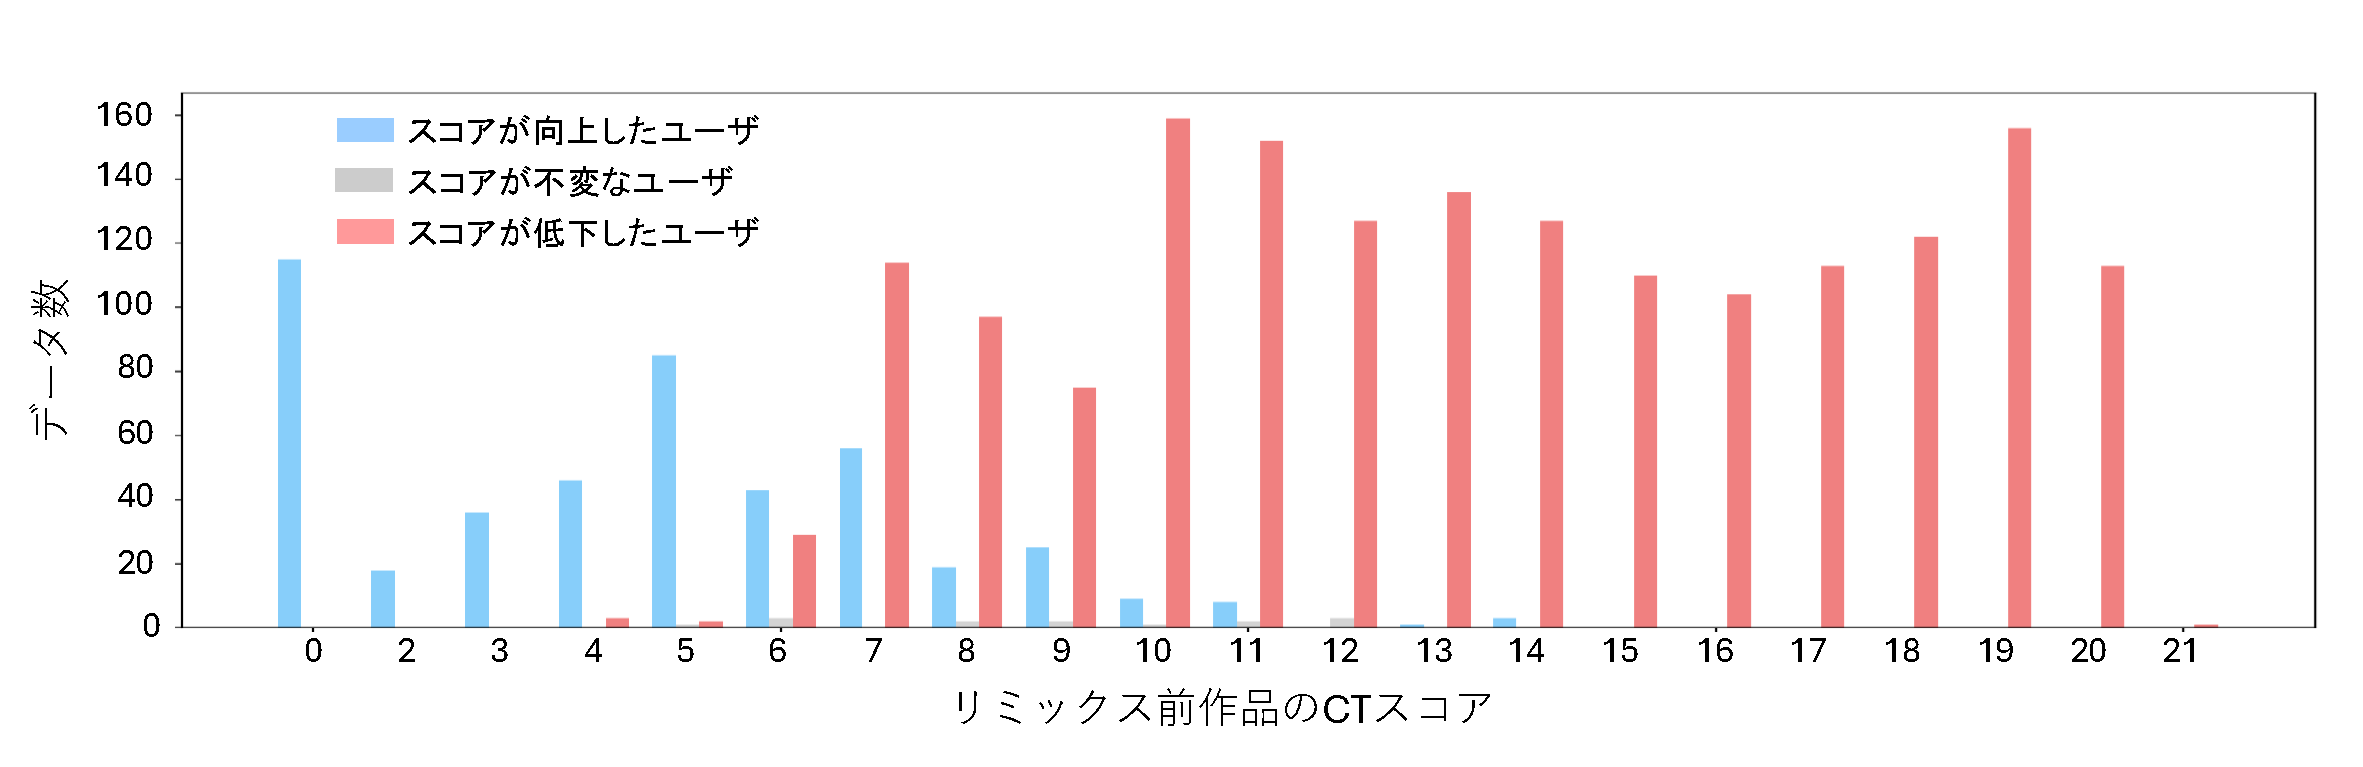
\includegraphics[width=\linewidth]{@IPSJ_SIGSE202511_Horio/fig/diffdata.pdf}
  \caption{テストデータにおいて予測により向上,不変,低下したユーザ数}
  \label{diffdata}
\end{figure}

\begin{figure}[h]
  \centering
  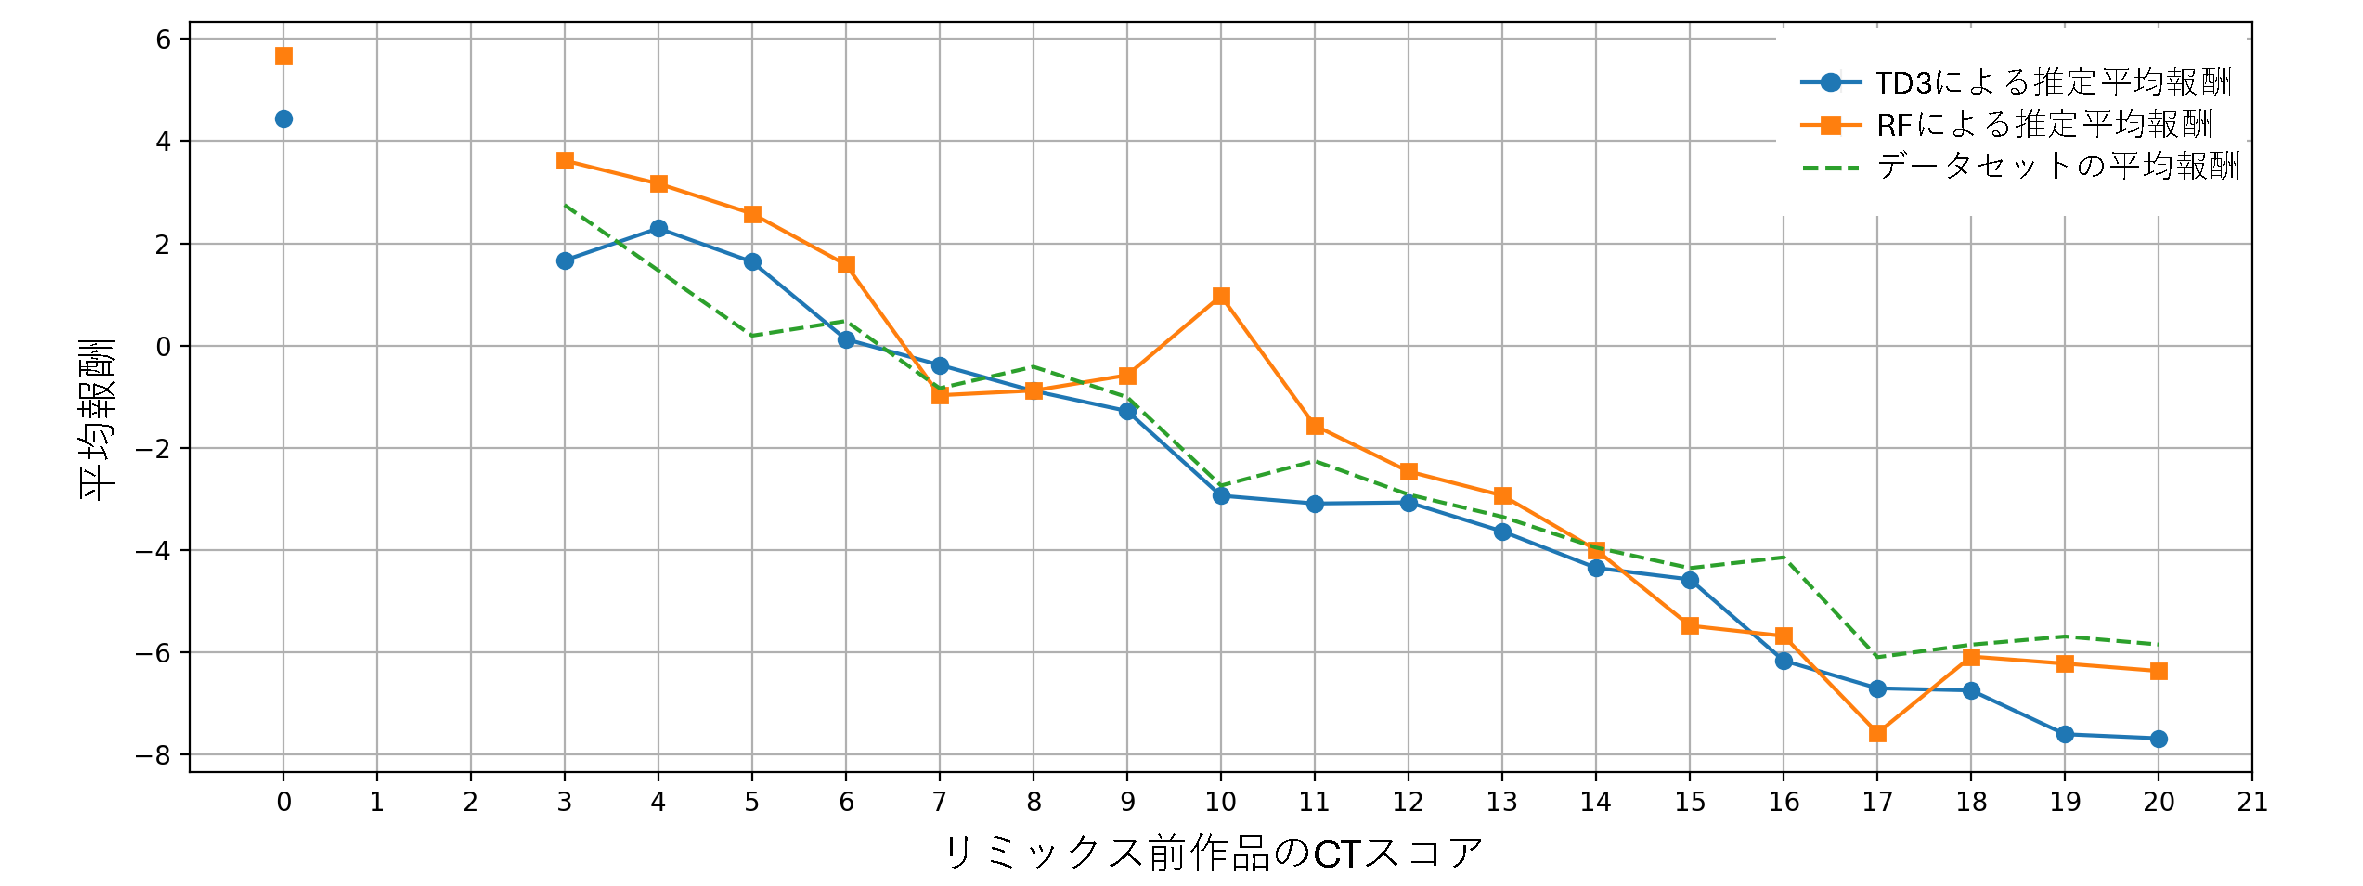
\includegraphics[width=\linewidth]{@IPSJ_SIGSE202511_Horio/fig/estgraph.pdf}
  \caption{強化学習モデルと教師あり学習の推定平均報酬グラフ}
  \label{estgraph}
\end{figure}
\begin{figure}[h]
  \centering
  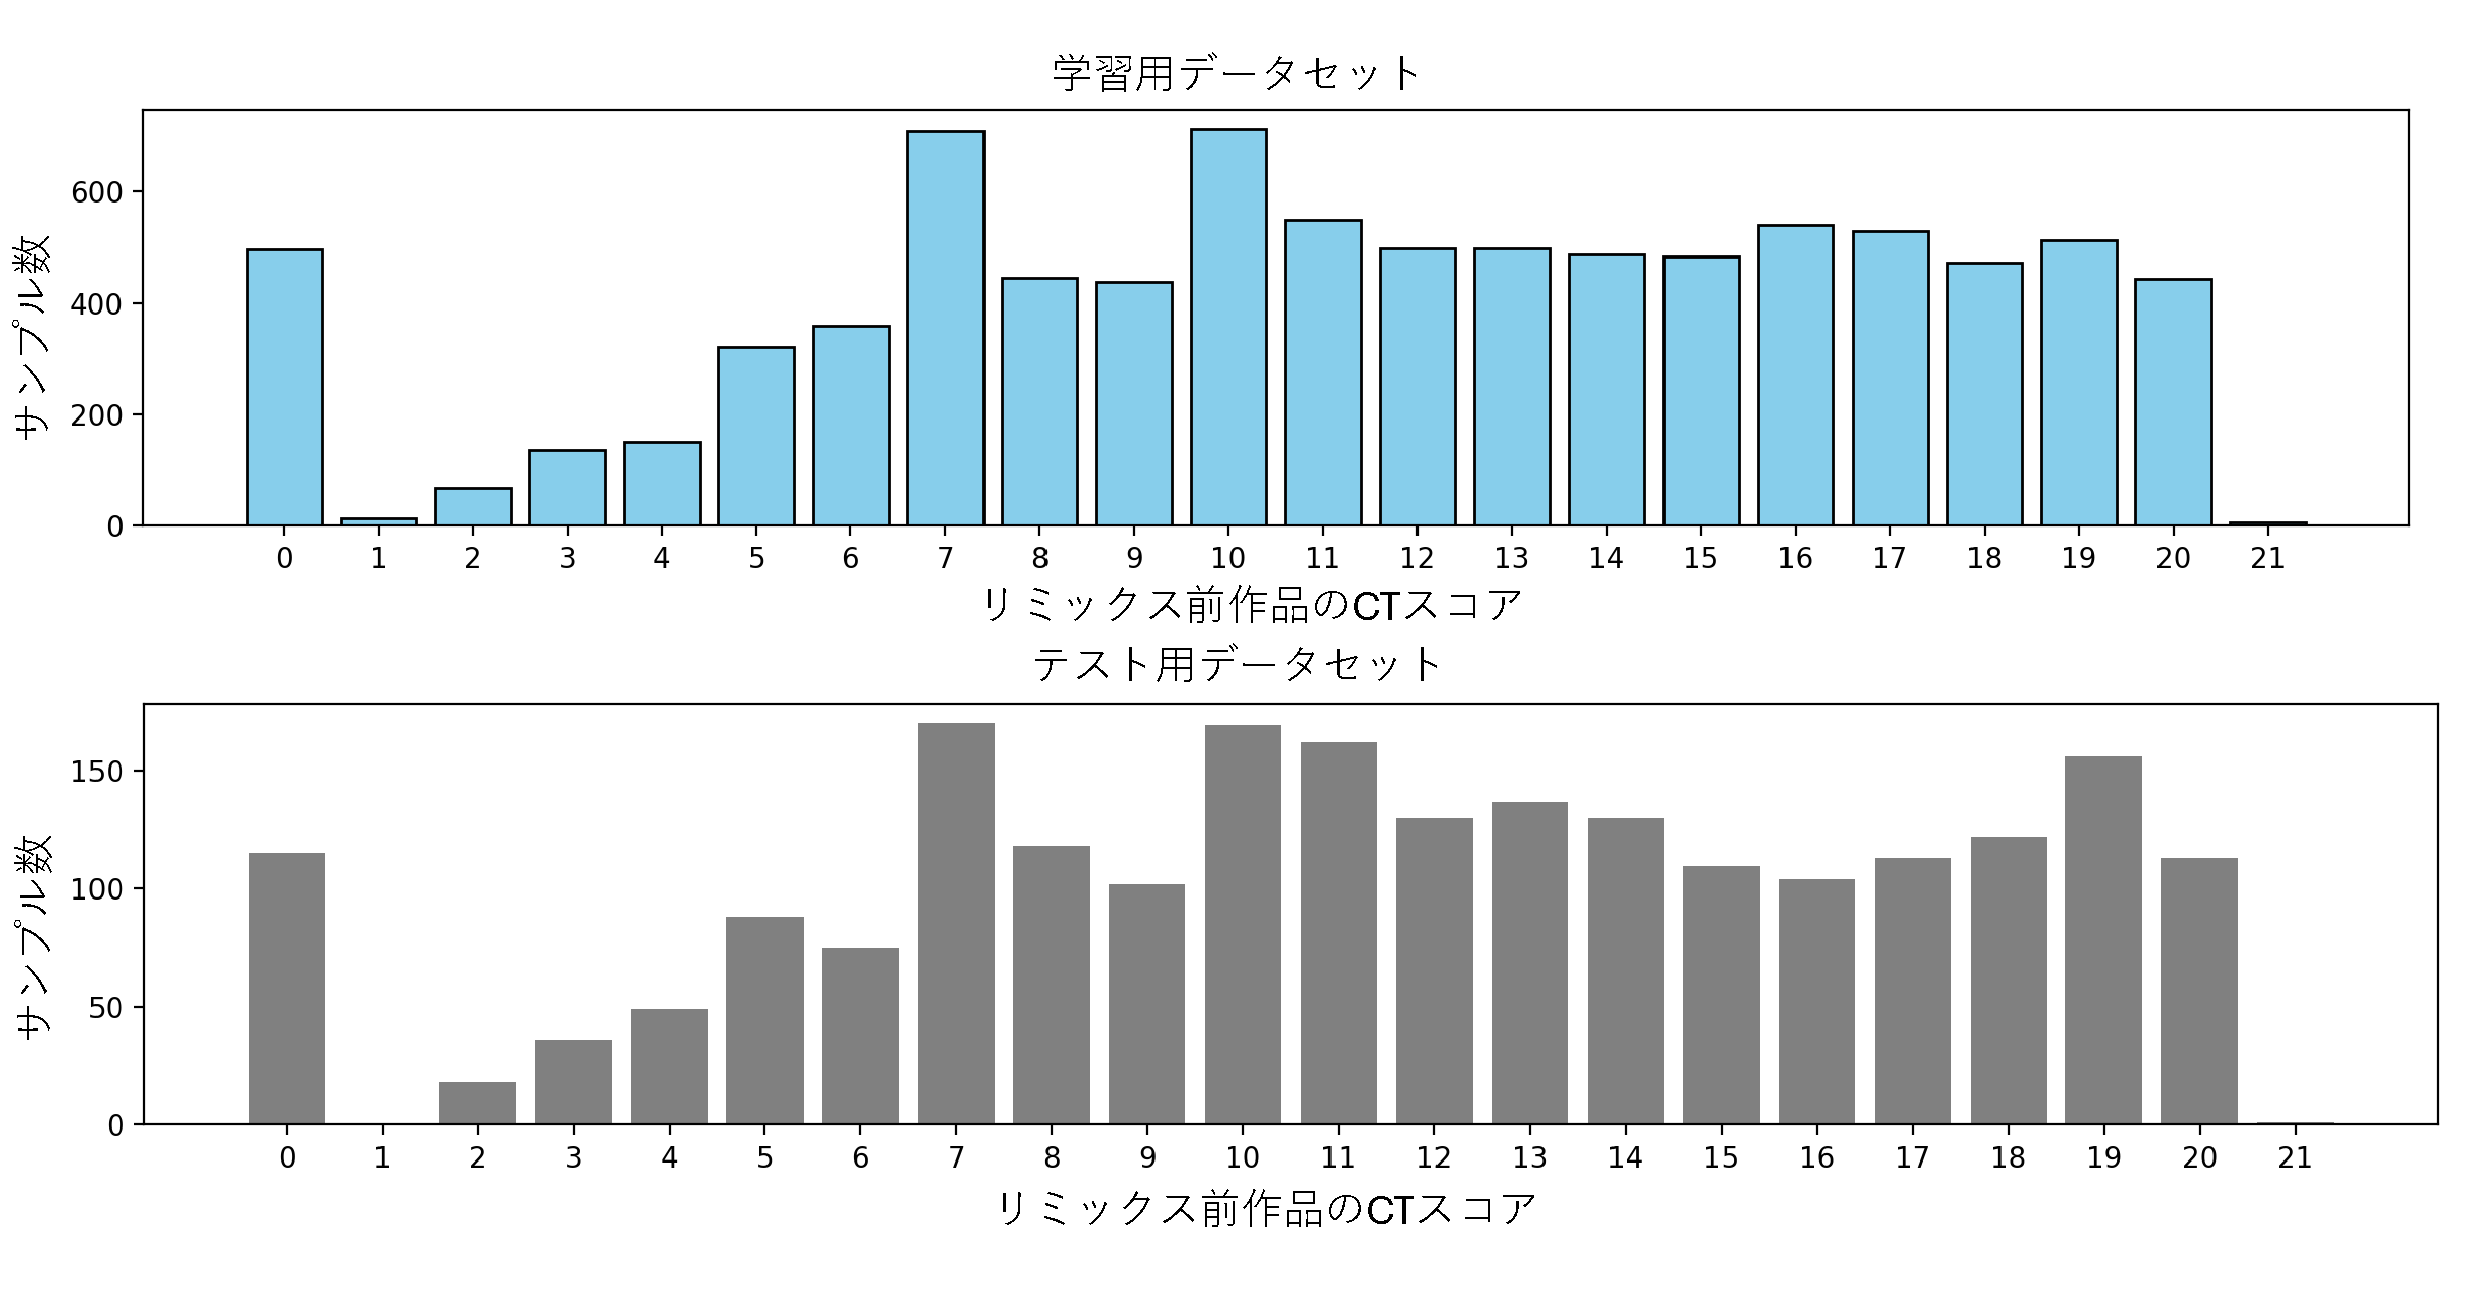
\includegraphics[width=\linewidth]{@IPSJ_SIGSE202511_Horio/fig/train_testdata.pdf}
  \caption{学習データとテストデータのリミックス前作品CTスコア分布}
  \label{train_testdata}
\end{figure}

図\ref{diffminigraph}は概念別にテストデータセットと予測データのリミックス元作品のCT概念スコア差を箱ひげ図で示したものであり,抽象化,同期,論理以外の概念は抽象化と似た図になったため省略している.また,図\ref{diffdata}はテストデータセットにおいて熟練度別のユーザ数を予測結果に基づいて棒グラフで示している.

図\ref{diffminigraph}を見ると,抽象化では実データよりも高いスコアのリミックス元作品を予測しているが,同期では低いスコアのリミックス元作品を予測している.また,論理ではほとんどの向上しているユーザは実データよりも高いスコアのリミックス元作品を予測した場合である.したがって,CTスコアを向上させるためのリミックス元作品の選択において,同期以外の概念のスコアは高い方が,同期のスコアは低い方が効果的であることが示唆される.

加えて,図\ref{diffdata}を見るとリミックス前作品のCTスコアが7点前後から,CTスコアが低下したユーザが増加してきている.したがって,当モデルはCTスコアが7点未満のユーザに有用であることが示唆される.

図\ref{estgraph}は,強化学習モデルと教師あり学習モデルによる推定平均報酬の結果を示す.横軸はリミックス前作品のCTスコア,縦軸は平均報酬を示す.青色線,橙色線,緑色線はそれぞれTD3による推定平均報酬,RFによる推定平均報酬,データセットの平均報酬を示す.リミックス元作品のCTスコアが1点,2点では,他CTスコアと比べてサンプル数が少ないため図\ref{estgraph}のグラフ上に描写していない.データ量と学習安定性の関係をみるため,図\ref{train_testdata}に学習データとテストデータのリミックス前作品CTスコアの分布を示す.

% 強化学習モデルと教師あり学習モデルによる推定平均報酬の結果を図\ref{estgraph},学習データとテストデータのリミックス前作品CTスコアの分布を図\ref{train_testdata}に示す.
% リミックス元作品のCTスコアが1点,2点では,他スコアと比べてサンプル数が少ないため図\ref{estgraph}のグラフ上には描写していない.

図\ref{estgraph}を見ると,強化学習モデルの推定平均報酬は,リミックス前作品のCTスコアが3点,6点でデータセットの平均報酬より少し下回るものの,6点まではデータセットの平均報酬よりも上回っており,また,0点以上の推定平均報酬になっている.しかし,CTスコアが7点以上では,データセットの平均報酬よりも下回っている部分が多く,また,推定平均報酬が0点未満である.

RFと比較すると,TD3は下回っているように見えるが,これは過大評価を抑制するTD3の本来の性質が影響している.また,RFはノイズや外れ値の影響を受けやすく,不安定である.

\subsection{考察}
強化学習モデルは6点までは基本的に平均報酬がデータセットよりも上回っていることや,推定平均報酬が0点以上になっていることから,強化学習モデルによる方策は初級者のCTスコア向上に有効である.
しかし,中級者以上はデータセットよりも下回っており,また推定平均報酬が0点以下になってしまっていることから,有効な方策とはいえない.そのため,熟練度によってモデルを分類する必要性も考えられる.

加えて,CTスコア向上に効果があるリミックス元作品のCT概念が同期以外であることが示唆された.RQ1の結果においても同期はリミックス前後作品で大きな差がみられなかったことから,リミックスにより同期のスコアを向上することが困難であることが考えられる.

また,リミックス前作品のスコアが1点,2点,3点,4点あたりのデータは非常に少なくなっており,どの熟練度にも対応することができるように,データセットを増やす必要性がある.他にも,TD3の強みである連続的な遷移の学習をもとに予測を行うために,オリジナル作品の制作過程を含む全遷移の学習モデルと今回構築したモデルを組み合わせ,2つのモデルで推薦する必要性が示唆される.加えて,今回は評価指標として推定平均報酬を用いたが,強化学習は環境の影響が大きく,固定データセットでは環境変化への適応や意思決定過程を評価できない.そのため,将来的にはシミュレータを作成し,評価する必要がある.


%%%%%%%%%%%%%%%%%%%%%%%%%%%
\section{おわりに}
\label{sec:conclusion}
%%%%%%%%%%%%%%%%%%%%%%%%%%%
本研究では,ユーザの熟練度とリミックス作品の関係を分析し,作品制作過程をマルコフ決定過程として捉えることで,強化学習に基づくユーザのCTスキルが向上するリミックス元作品のCTスコア予測モデルを構築した.
評価の結果,提案したモデルは初級者におけるCTスコア向上に有効であることを確認したが,中級者以上のユーザには十分な効果が得られなかった.

本研究の妥当性を評価するにあたり,主に以下の2点の可能性について検討し,それに対する対策を講じた.オリジナル作品の制作を重ねることにより,CTスコアが向上した可能性がある.本研究ではリミックス直後に制作したオリジナル作品3件をリミックス後作品の対象とすることで,脅威を軽減する.また,リミックスを介さずにほかユーザの作品を模倣して制作した作品や,他ユーザのアカウントを使用して制作した作品,他ユーザが支援を行って制作した作品が存在する可能性がある.このような作品がデータセットに混ざっている場合,分析に違いが生じることが考えられる.本研究ではリミックスを行ったことがあるユーザに限定し,多くのデータセットを用意することで,脅威となるような作品の影響を軽減する.

今後はデータセットを拡充し,ユーザの熟練度に応じてモデルを分類することで,予測精度の向上を図る.また,リミックス遷移だけでなく,作品制作過程全体の状態遷移を学習対象とし,予測を行うことで,強化学習の特性をより活かした予測を実現できると考える.また,CT概念の学習順を考慮する必要性も考えられる.

% データセット不足による学習の不安定さが考えられる.
% 熟練度によってモデルを分類する必要性が示唆される.
% モデルの精度予測のため,シミュレータの作成も必要になると考える.


\bibliographystyle{unsrt}
\bibliography{references}

\end{document}
